% Options for packages loaded elsewhere
\PassOptionsToPackage{unicode}{hyperref}
\PassOptionsToPackage{hyphens}{url}
%
\documentclass[
  ignorenonframetext,
]{beamer}
\usepackage{pgfpages}
\setbeamertemplate{caption}[numbered]
\setbeamertemplate{caption label separator}{: }
\setbeamercolor{caption name}{fg=normal text.fg}
\beamertemplatenavigationsymbolsempty
% Prevent slide breaks in the middle of a paragraph
\widowpenalties 1 10000
\raggedbottom
\setbeamertemplate{part page}{
  \centering
  \begin{beamercolorbox}[sep=16pt,center]{part title}
    \usebeamerfont{part title}\insertpart\par
  \end{beamercolorbox}
}
\setbeamertemplate{section page}{
  \centering
  \begin{beamercolorbox}[sep=12pt,center]{part title}
    \usebeamerfont{section title}\insertsection\par
  \end{beamercolorbox}
}
\setbeamertemplate{subsection page}{
  \centering
  \begin{beamercolorbox}[sep=8pt,center]{part title}
    \usebeamerfont{subsection title}\insertsubsection\par
  \end{beamercolorbox}
}
\AtBeginPart{
  \frame{\partpage}
}
\AtBeginSection{
  \ifbibliography
  \else
    \frame{\sectionpage}
  \fi
}
\AtBeginSubsection{
  \frame{\subsectionpage}
}

\usepackage{amsmath,amssymb}
\usepackage{iftex}
\ifPDFTeX
  \usepackage[T1]{fontenc}
  \usepackage[utf8]{inputenc}
  \usepackage{textcomp} % provide euro and other symbols
\else % if luatex or xetex
  \usepackage{unicode-math}
  \defaultfontfeatures{Scale=MatchLowercase}
  \defaultfontfeatures[\rmfamily]{Ligatures=TeX,Scale=1}
\fi
\usepackage{lmodern}
\usetheme[]{Singapore}
\ifPDFTeX\else  
    % xetex/luatex font selection
\fi
% Use upquote if available, for straight quotes in verbatim environments
\IfFileExists{upquote.sty}{\usepackage{upquote}}{}
\IfFileExists{microtype.sty}{% use microtype if available
  \usepackage[]{microtype}
  \UseMicrotypeSet[protrusion]{basicmath} % disable protrusion for tt fonts
}{}
\makeatletter
\@ifundefined{KOMAClassName}{% if non-KOMA class
  \IfFileExists{parskip.sty}{%
    \usepackage{parskip}
  }{% else
    \setlength{\parindent}{0pt}
    \setlength{\parskip}{6pt plus 2pt minus 1pt}}
}{% if KOMA class
  \KOMAoptions{parskip=half}}
\makeatother
\usepackage{xcolor}
\newif\ifbibliography
\setlength{\emergencystretch}{3em} % prevent overfull lines
\setcounter{secnumdepth}{-\maxdimen} % remove section numbering


\providecommand{\tightlist}{%
  \setlength{\itemsep}{0pt}\setlength{\parskip}{0pt}}\usepackage{longtable,booktabs,array}
\usepackage{calc} % for calculating minipage widths
\usepackage{caption}
% Make caption package work with longtable
\makeatletter
\def\fnum@table{\tablename~\thetable}
\makeatother
\usepackage{graphicx}
\makeatletter
\def\maxwidth{\ifdim\Gin@nat@width>\linewidth\linewidth\else\Gin@nat@width\fi}
\def\maxheight{\ifdim\Gin@nat@height>\textheight\textheight\else\Gin@nat@height\fi}
\makeatother
% Scale images if necessary, so that they will not overflow the page
% margins by default, and it is still possible to overwrite the defaults
% using explicit options in \includegraphics[width, height, ...]{}
\setkeys{Gin}{width=\maxwidth,height=\maxheight,keepaspectratio}
% Set default figure placement to htbp
\makeatletter
\def\fps@figure{htbp}
\makeatother

\titlegraphic{
\includegraphics[width=3cm]{../20240214_SOT_ISES_Webinar/set-logo.jpg}}
\setbeamertemplate{frametitle continuation}[from second]
\makeatletter
\@ifpackageloaded{caption}{}{\usepackage{caption}}
\AtBeginDocument{%
\ifdefined\contentsname
  \renewcommand*\contentsname{Table of contents}
\else
  \newcommand\contentsname{Table of contents}
\fi
\ifdefined\listfigurename
  \renewcommand*\listfigurename{List of Figures}
\else
  \newcommand\listfigurename{List of Figures}
\fi
\ifdefined\listtablename
  \renewcommand*\listtablename{List of Tables}
\else
  \newcommand\listtablename{List of Tables}
\fi
\ifdefined\figurename
  \renewcommand*\figurename{Figure}
\else
  \newcommand\figurename{Figure}
\fi
\ifdefined\tablename
  \renewcommand*\tablename{Table}
\else
  \newcommand\tablename{Table}
\fi
}
\@ifpackageloaded{float}{}{\usepackage{float}}
\floatstyle{ruled}
\@ifundefined{c@chapter}{\newfloat{codelisting}{h}{lop}}{\newfloat{codelisting}{h}{lop}[chapter]}
\floatname{codelisting}{Listing}
\newcommand*\listoflistings{\listof{codelisting}{List of Listings}}
\makeatother
\makeatletter
\makeatother
\makeatletter
\@ifpackageloaded{caption}{}{\usepackage{caption}}
\@ifpackageloaded{subcaption}{}{\usepackage{subcaption}}
\makeatother
\ifLuaTeX
  \usepackage{selnolig}  % disable illegal ligatures
\fi
\usepackage{bookmark}

\IfFileExists{xurl.sty}{\usepackage{xurl}}{} % add URL line breaks if available
\urlstyle{same} % disable monospaced font for URLs
\hypersetup{
  pdftitle={Geospatial Methodologies in Toxicology},
  pdfauthor={Kyle P Messier, PhD},
  hidelinks,
  pdfcreator={LaTeX via pandoc}}

\title{Geospatial Methodologies in Toxicology}
\subtitle{Linking exposure, toxicity, and disease profiles to identify
U.S. regions at elevated health risks}
\author{Kyle P Messier, PhD}
\date{}
\institute{National Institute of Environmental Health Sciences -
Division of Translational Toxicology - Predictive Toxicology Branch}

\begin{document}
\frame{\titlepage}

\section{Introduction}\label{introduction}

\begin{frame}{About Us}
\phantomsection\label{about-us}
\textbf{Spatiotemporal Exposures and Toxicology \{SET\} group}

\begin{columns}[T]
\begin{column}{0.5\textwidth}
\begin{itemize}
\tightlist
\item
  Spatiotemporal Exposure Mapping
\item
  Chemical and Stressor Mixtures Prediction
\item
  Mechanistically Informed Geospatial Risk Assessment
\end{itemize}
\end{column}

\begin{column}{0.5\textwidth}
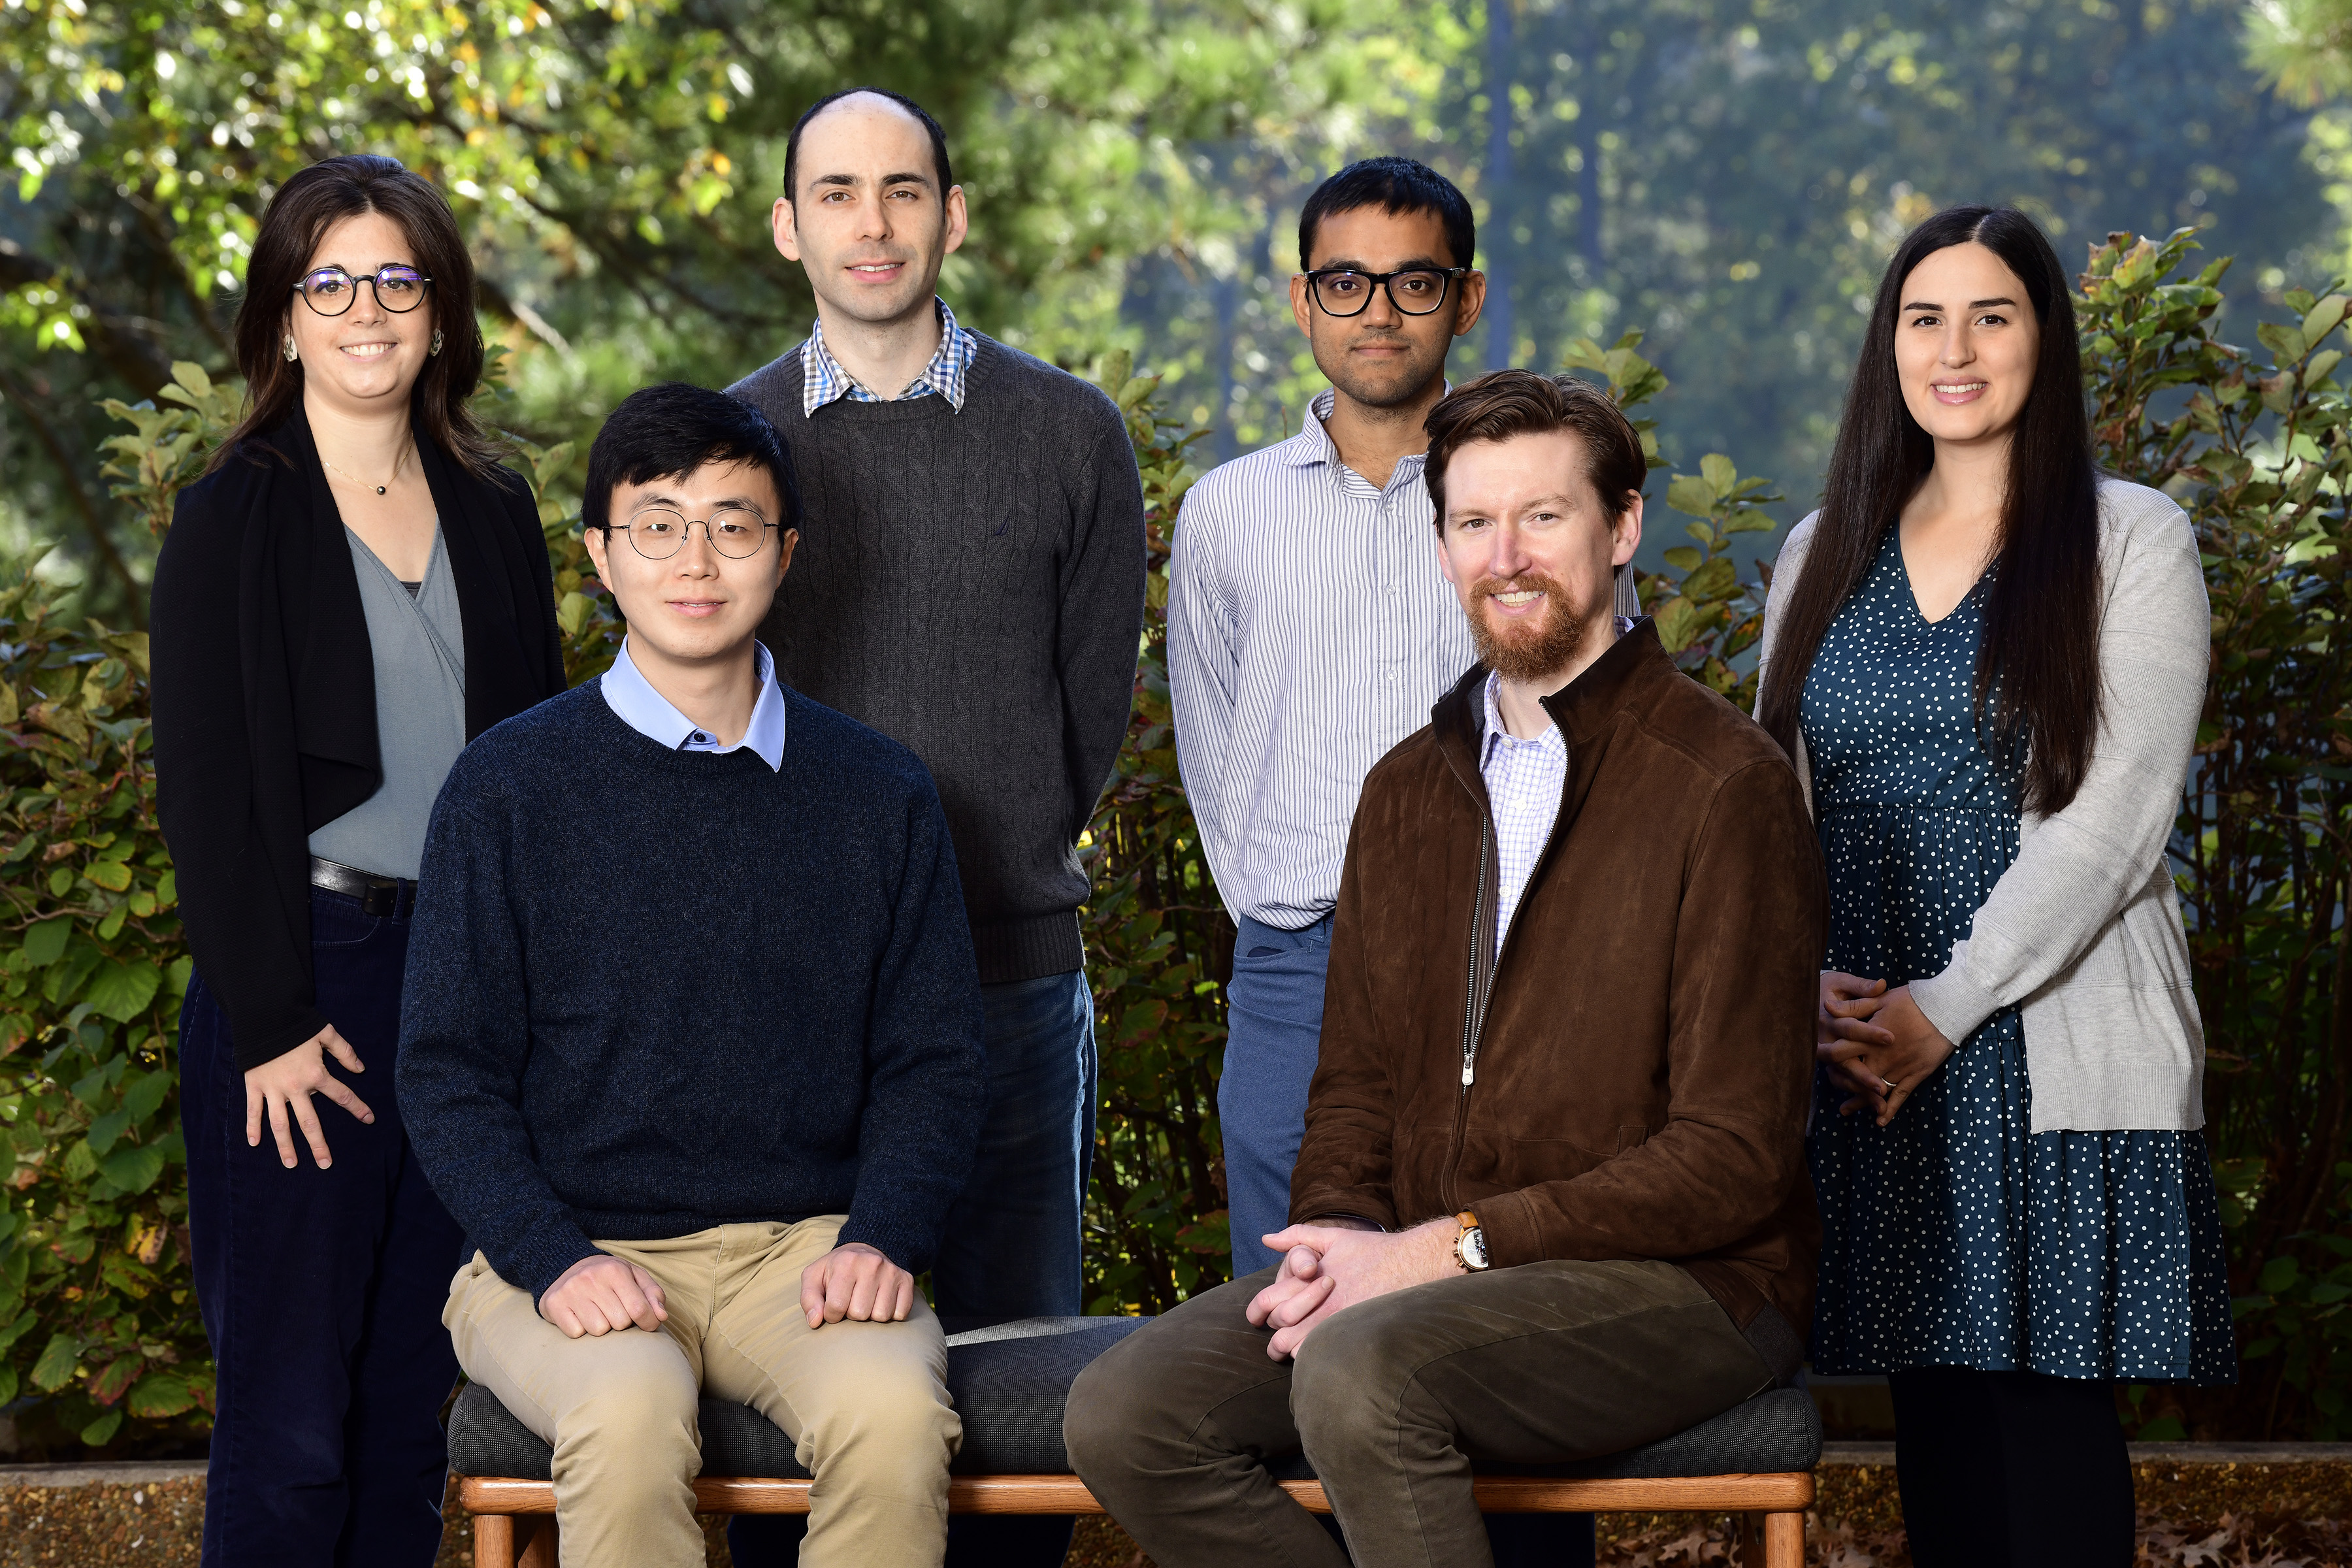
\includegraphics{../../presentations/20240222_UNC_ESE_Guest_Lecture/SETgroup-Oct2023.jpg}
\end{column}
\end{columns}
\end{frame}

\begin{frame}{Geospatial Methods}
\phantomsection\label{geospatial-methods}
\begin{columns}[T]
\begin{column}{0.5\textwidth}
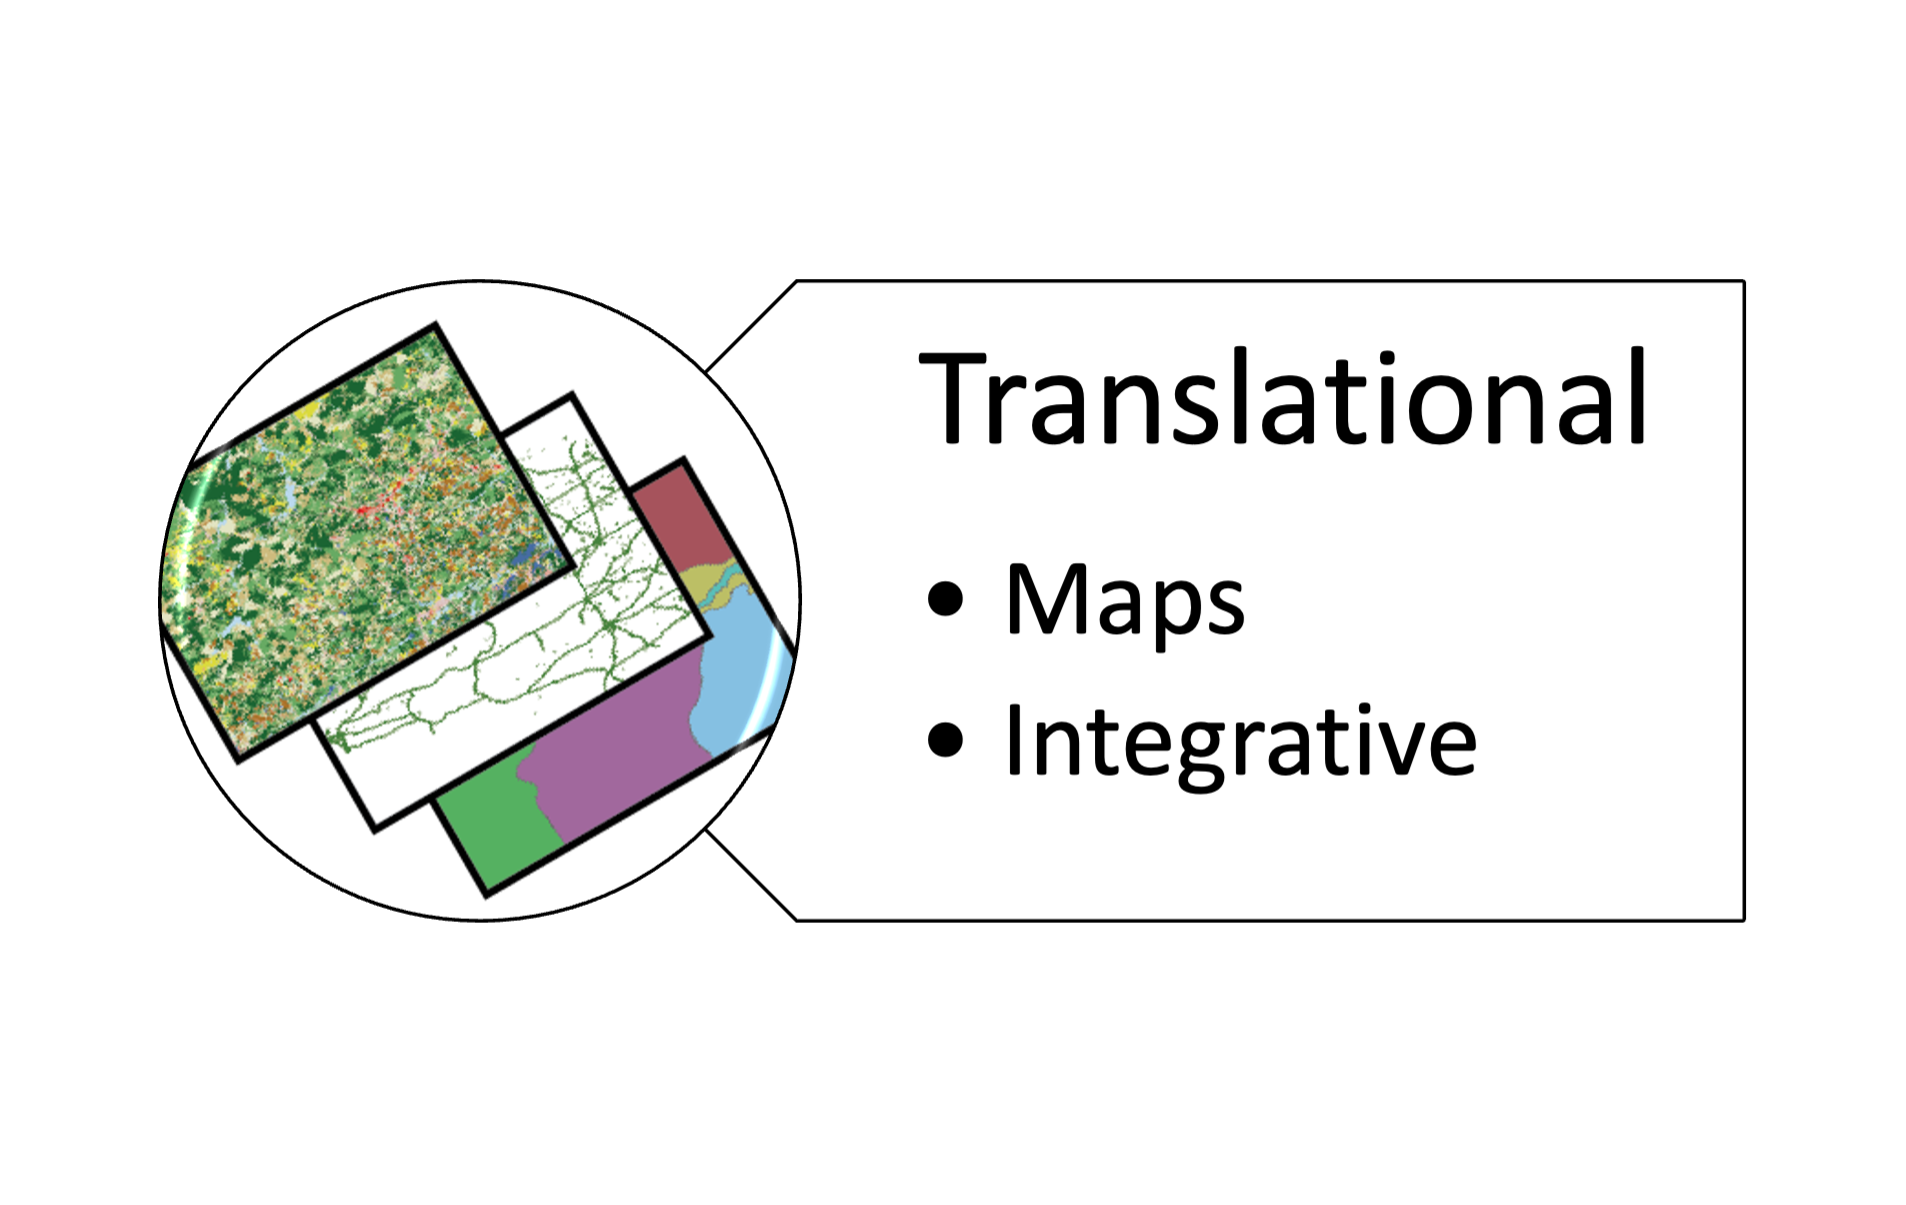
\includegraphics{../../presentations/20240222_UNC_ESE_Guest_Lecture/maps-translational.png}
\end{column}

\begin{column}{0.5\textwidth}
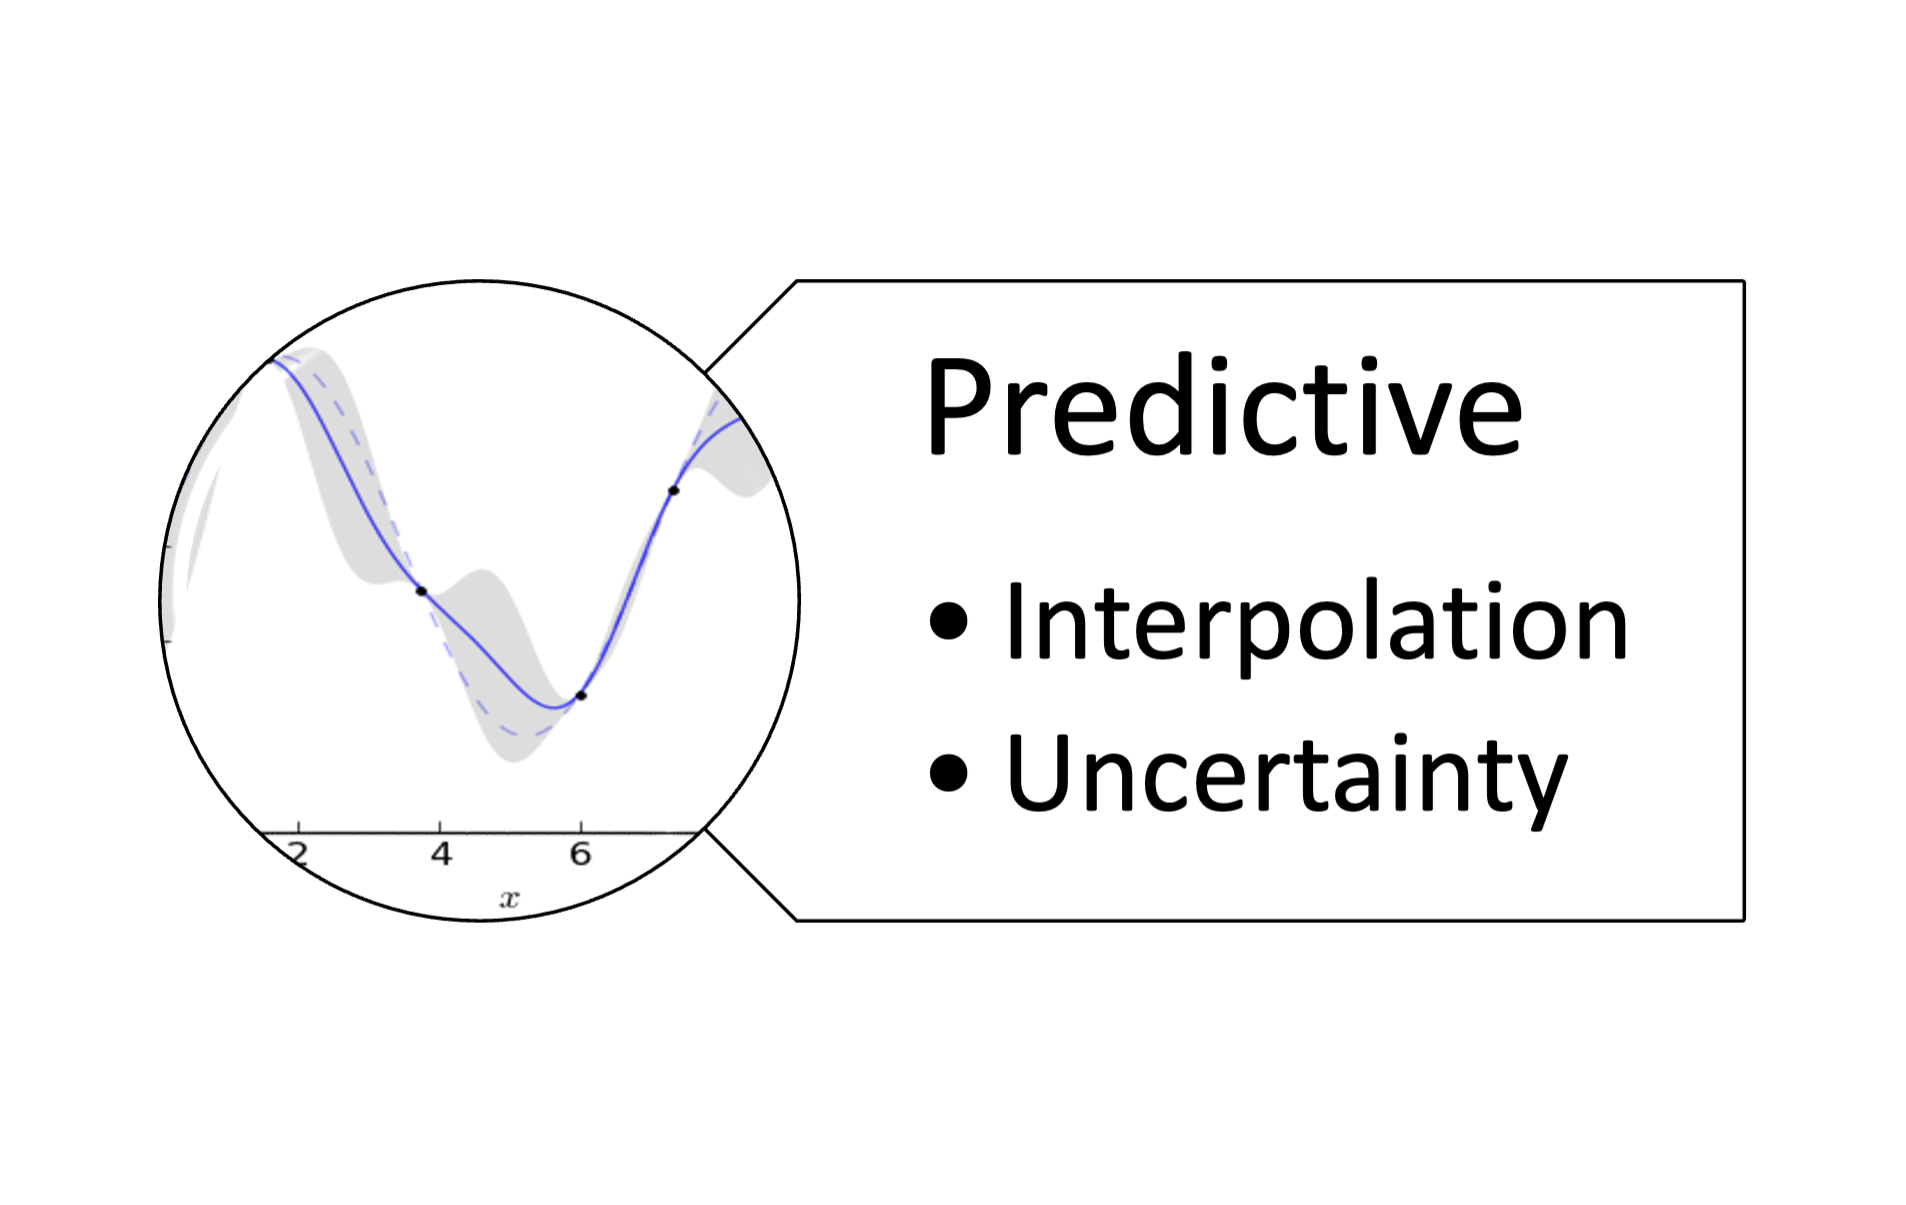
\includegraphics{../../presentations/20240222_UNC_ESE_Guest_Lecture/geostats-predictive.png}
\end{column}
\end{columns}
\end{frame}

\begin{frame}{Objective}
\phantomsection\label{objective}
\begin{itemize}
\tightlist
\item
  Provide an overview of geospatial methods, data, applications, and
  future directions in toxicology and risk assessment
\end{itemize}
\end{frame}

\section{History}\label{history}

\begin{frame}{Mining}
\phantomsection\label{mining}
\begin{columns}[T]
\begin{column}{0.5\textwidth}
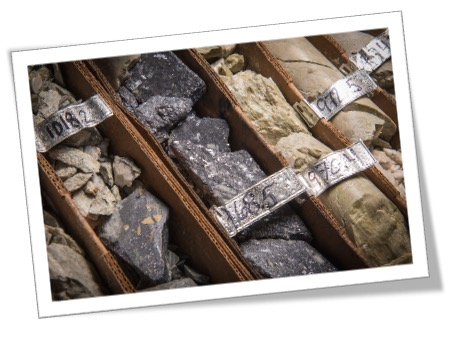
\includegraphics{../../presentations/20240222_UNC_ESE_Guest_Lecture/mining.jpg}
\end{column}

\begin{column}{0.5\textwidth}
\begin{itemize}
\tightlist
\item
  Matheron and Krige developed geostatistical methods to predict ore
  content from core samples
\item
  Matheron coined the term ``Kriging'' after Krige
\item
  ``Nugget'' is a term used to random noise because predicting where
  gold nuggets were was so difficult
\end{itemize}
\end{column}
\end{columns}
\end{frame}

\begin{frame}{Forestry}
\phantomsection\label{forestry}
\begin{columns}[T]
\begin{column}{0.5\textwidth}
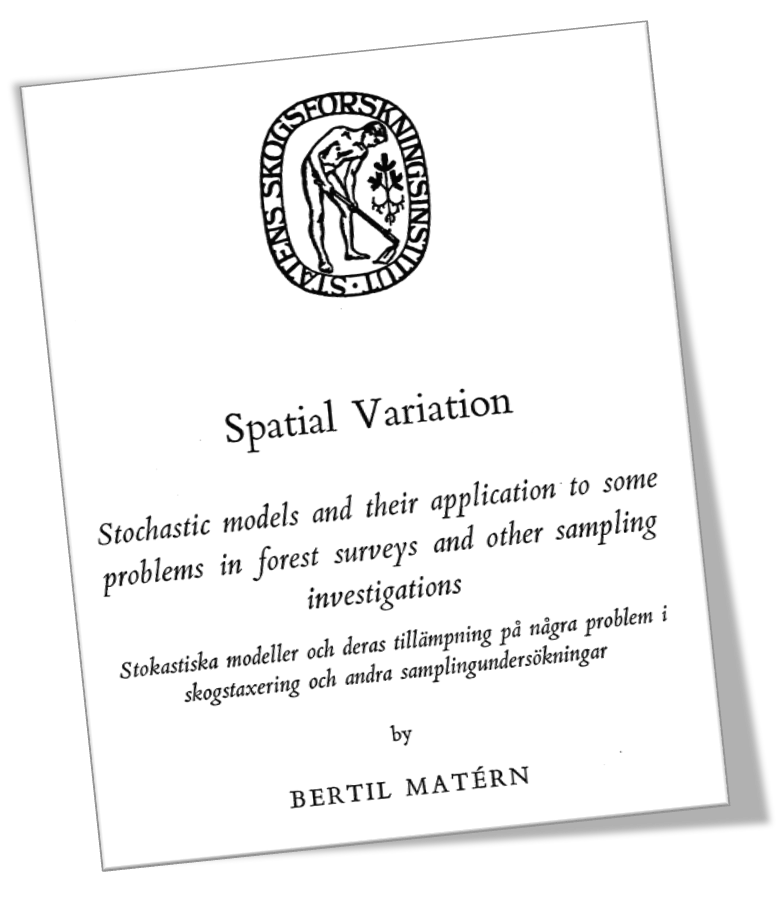
\includegraphics{../../presentations/20240222_UNC_ESE_Guest_Lecture/matern.png}
\end{column}

\begin{column}{0.5\textwidth}
\begin{itemize}
\tightlist
\item
  Matérn developed correlation models for spatial variation for
  applications in Forestry
\item
  To this day, we use the ``Matérn'' covariance function
\end{itemize}
\end{column}
\end{columns}
\end{frame}

\begin{frame}{Petroleum Engineering}
\phantomsection\label{petroleum-engineering}
\begin{columns}[T]
\begin{column}{0.6\textwidth}
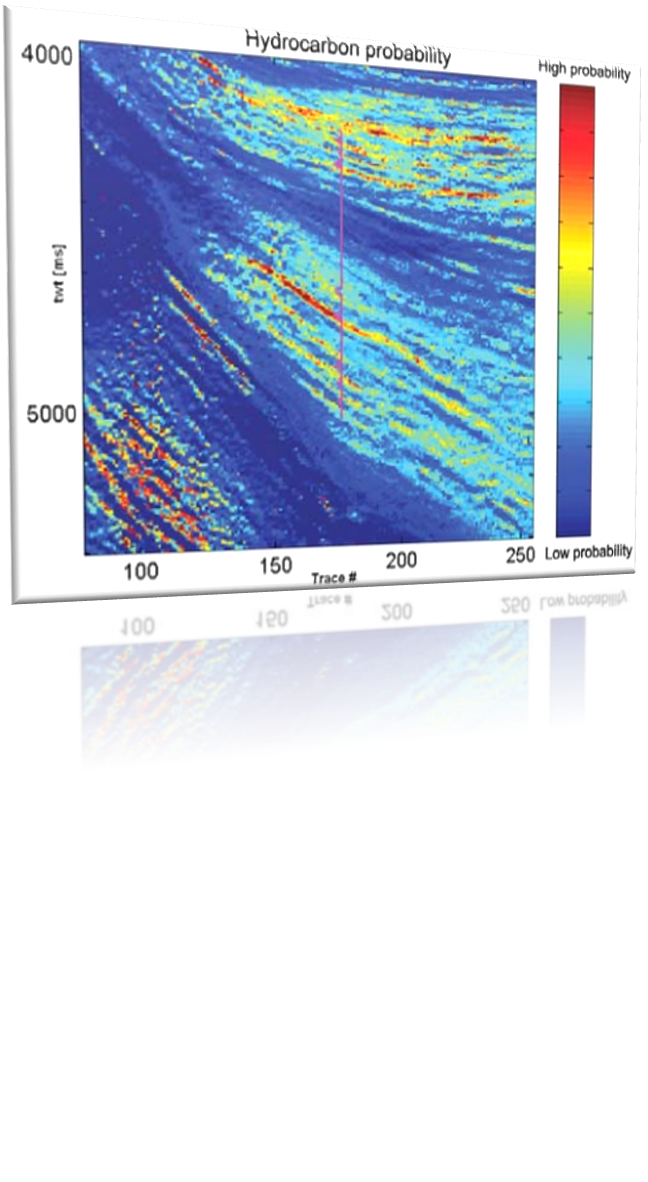
\includegraphics[width=0.6\textwidth,height=\textheight]{../../presentations/20240222_UNC_ESE_Guest_Lecture/petroleum.png}
\end{column}

\begin{column}{0.4\textwidth}
\begin{itemize}
\tightlist
\item
  Used to evaluate the oil and gas field reservoirs
\item
  Uses geology and seismic data
\end{itemize}
\end{column}
\end{columns}
\end{frame}

\begin{frame}{Public Health}
\phantomsection\label{public-health}
\begin{columns}[T]
\begin{column}{0.4\textwidth}
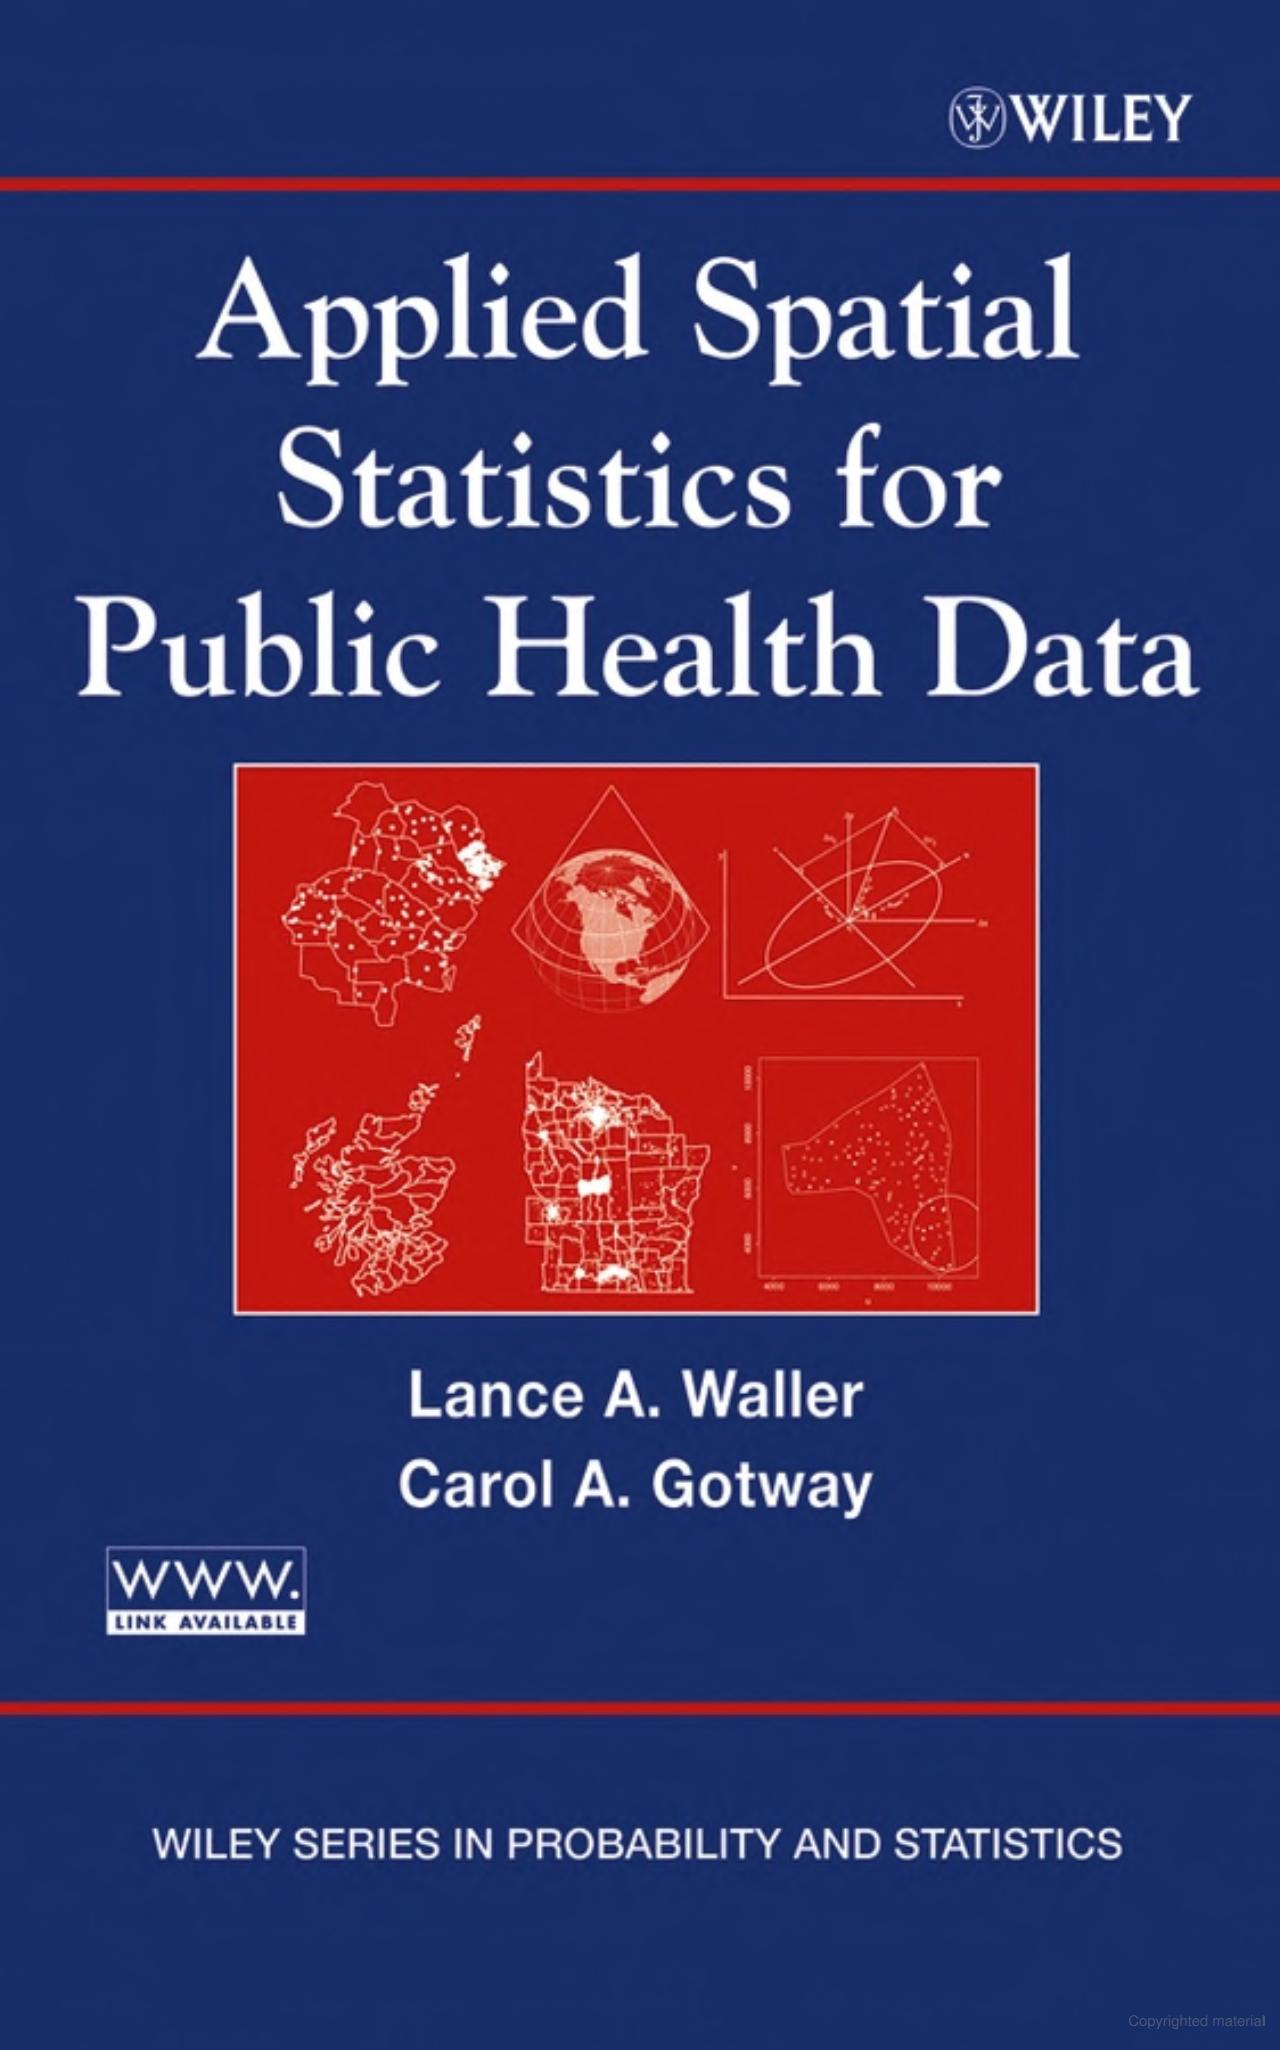
\includegraphics{../../presentations/20240222_UNC_ESE_Guest_Lecture/book-cover.jpeg}
\end{column}

\begin{column}{0.6\textwidth}
\begin{itemize}
\item
  Cressie, 1990: Statistics for Spatial Data
\item
  Waller and Gotway, 2004: Applied Statistics for Public Health Data
\item
  Wide scale adoption for statisticians and engineers in ecological and
  human exposure and risk applications
\end{itemize}
\end{column}
\end{columns}
\end{frame}

\begin{frame}{Toxicology}
\phantomsection\label{toxicology}
\begin{columns}[T]
\begin{column}{0.5\textwidth}
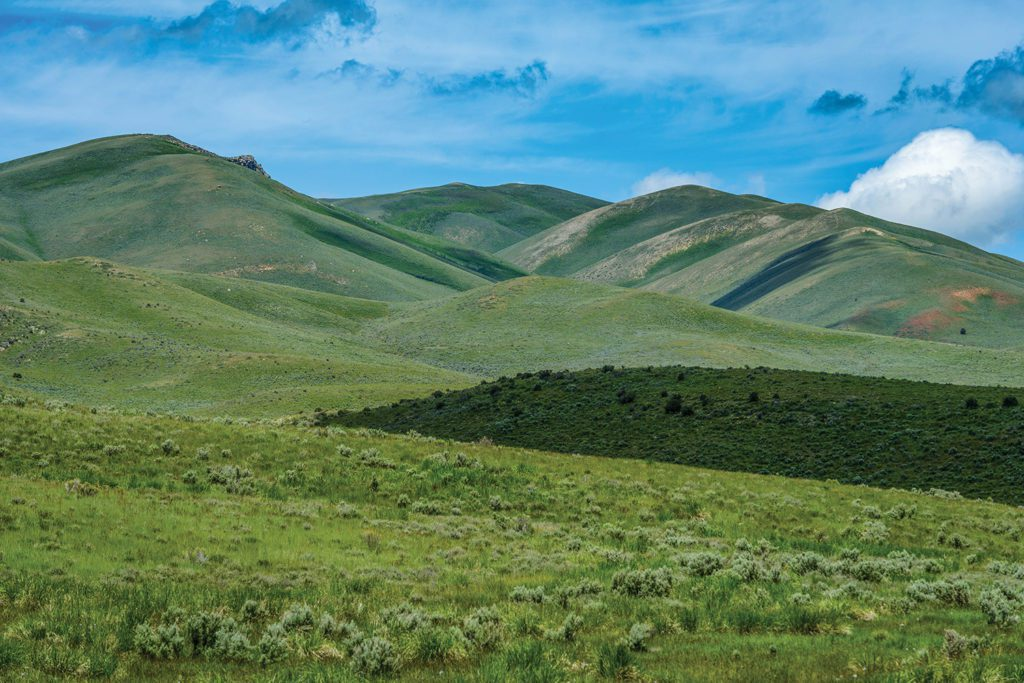
\includegraphics[width=0.97\textwidth,height=\textheight]{../20240311_SOT_Meeting_Talk/PublicLands.jpeg}
\end{column}

\begin{column}{0.5\textwidth}
\begin{itemize}
\item
  \textbf{Toxicology is a new frontier for geospatial methods}
\item
  Aggregate Exposure Pathways
\item
  Adverse Outcome Pathway
\item
  GeoTox
\item
  Source-to-Outcome
\end{itemize}
\end{column}
\end{columns}
\end{frame}

\section{Classical Models}\label{classical-models}

\begin{frame}{Uses in Public Health}
\phantomsection\label{uses-in-public-health}
\begin{itemize}
\item
  Estimate exposure to air pollutants, water contaminants, and other
  environmental stressors
\item
  Geocode patient addresses to link to environmental exposures
\item
  Estimate the spatial distribution of disease rates
\item
  Estimate the spatial distribution of health risk factors
\end{itemize}
\end{frame}

\begin{frame}{Land Use Regression}
\phantomsection\label{land-use-regression}
Linear regression for spatial data

\[
Y(s) =  X(s)\beta + \varepsilon
\]

where \(Y(s)\) is the response variable, \(X(s)\) are the predictor
variables, \(\beta\) are the regression coefficients, \(\varepsilon\) is
the iid error term, and \((s)\) denotes the spatial location.

Not a terrible idea for spatial data, but it directly violates the
assumption of independence of observations.
\end{frame}

\begin{frame}{Kriging}
\phantomsection\label{kriging}
Kriging and spatial models provide an explicit term for spatial
correlation. A reasonable approach is a random-effect model:

\[
Y(s) = \mu(s) + \varepsilon +  \eta(s)
\] where \(\eta \sim N_n(0,\Sigma_{\theta})\)

and \(\Sigma_{\theta}\) is a covariance matrix with parameters,
\(\theta\), that accounts for correlation between spatial and temporal
locations
\end{frame}

\section{Data Sources}\label{data-sources}

\begin{frame}{Common Data Sources and Types}
\phantomsection\label{common-data-sources-and-types}
\begin{columns}[T]
\begin{column}{0.5\textwidth}
\begin{itemize}
\tightlist
\item
  U.S. Census Bureau
\item
  U.S. Environmental Protection Agency
\item
  U.S. Geological Survey
\item
  National Aeronautics and Space Administration
\item
  National Oceanic and Atmospheric Administration
\item
  U.S. Department of Agriculture
\end{itemize}
\end{column}

\begin{column}{0.5\textwidth}
\begin{itemize}
\tightlist
\item
  Land cover data
\item
  Health statistics
\item
  Population characteristics
\item
  Infrastructure data
\item
  Air quality data
\item
  Water quality data
\item
  Satellite imagery
\end{itemize}
\end{column}
\end{columns}
\end{frame}

\begin{frame}{Satellite Imagery}
\phantomsection\label{satellite-imagery}
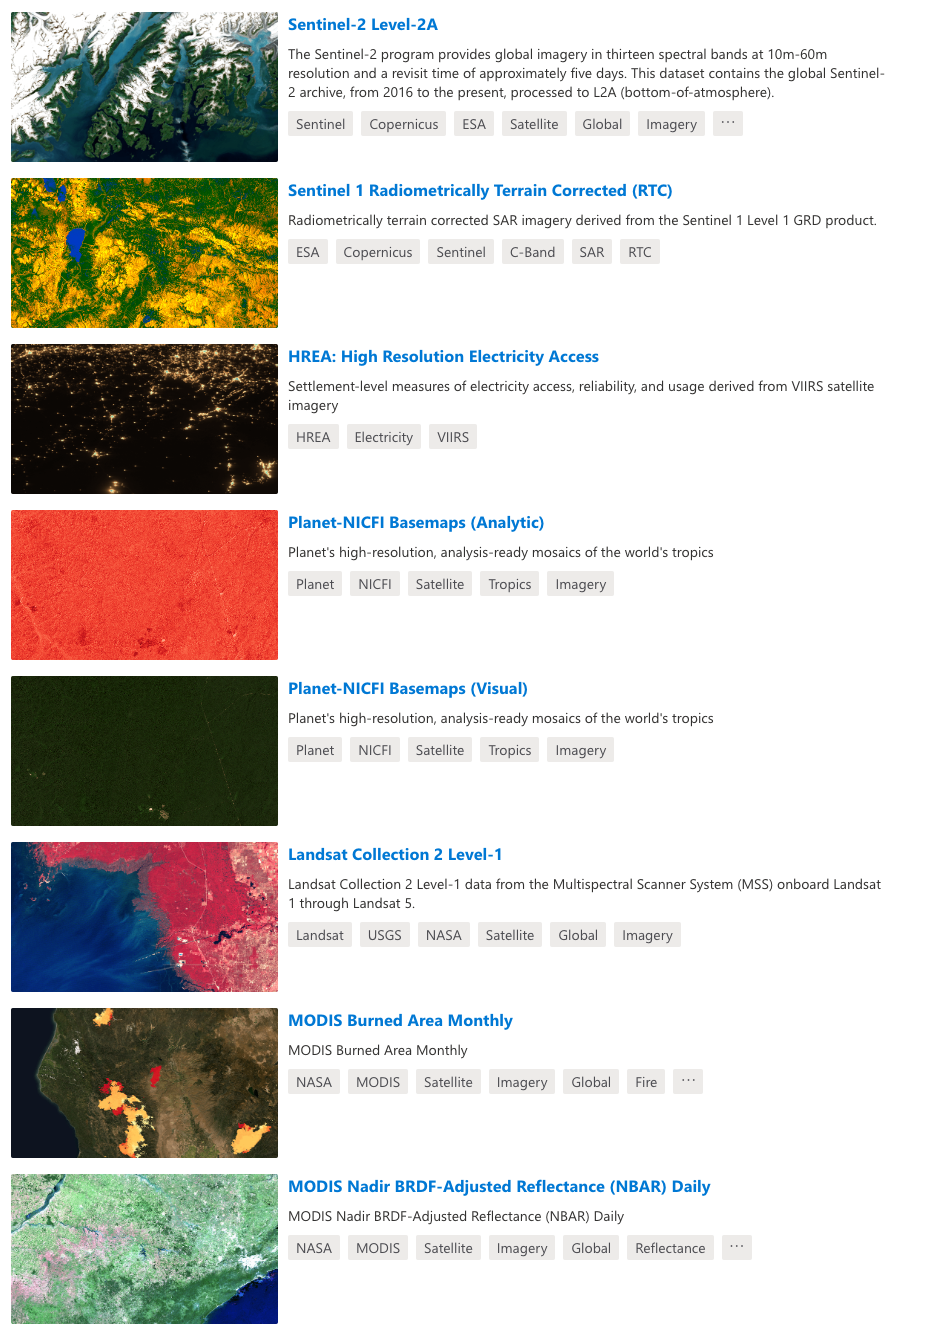
\includegraphics{satellite-data.png}
\end{frame}

\begin{frame}{Air Quality Data}
\phantomsection\label{air-quality-data}
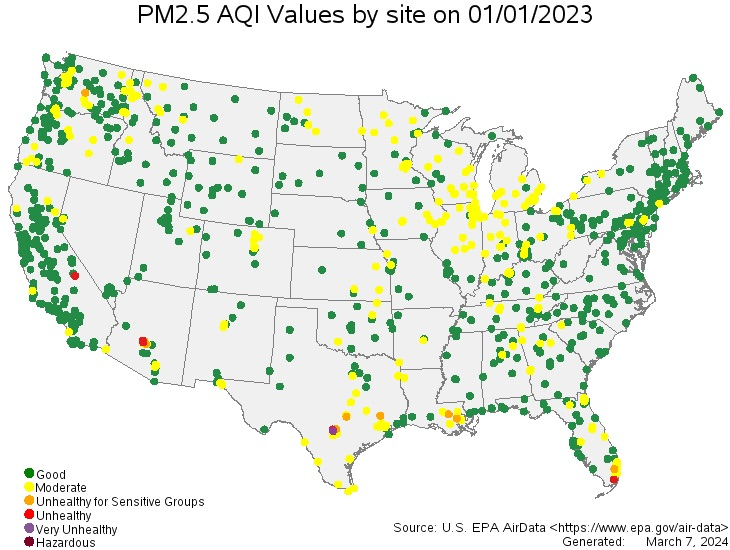
\includegraphics{AQI.jpeg}
\end{frame}

\begin{frame}{Toxic Release Data}
\phantomsection\label{toxic-release-data}
\includegraphics{TRI-utah.png}
\end{frame}

\begin{frame}{Health Information}
\phantomsection\label{health-information}
\begin{figure}[H]

{\centering 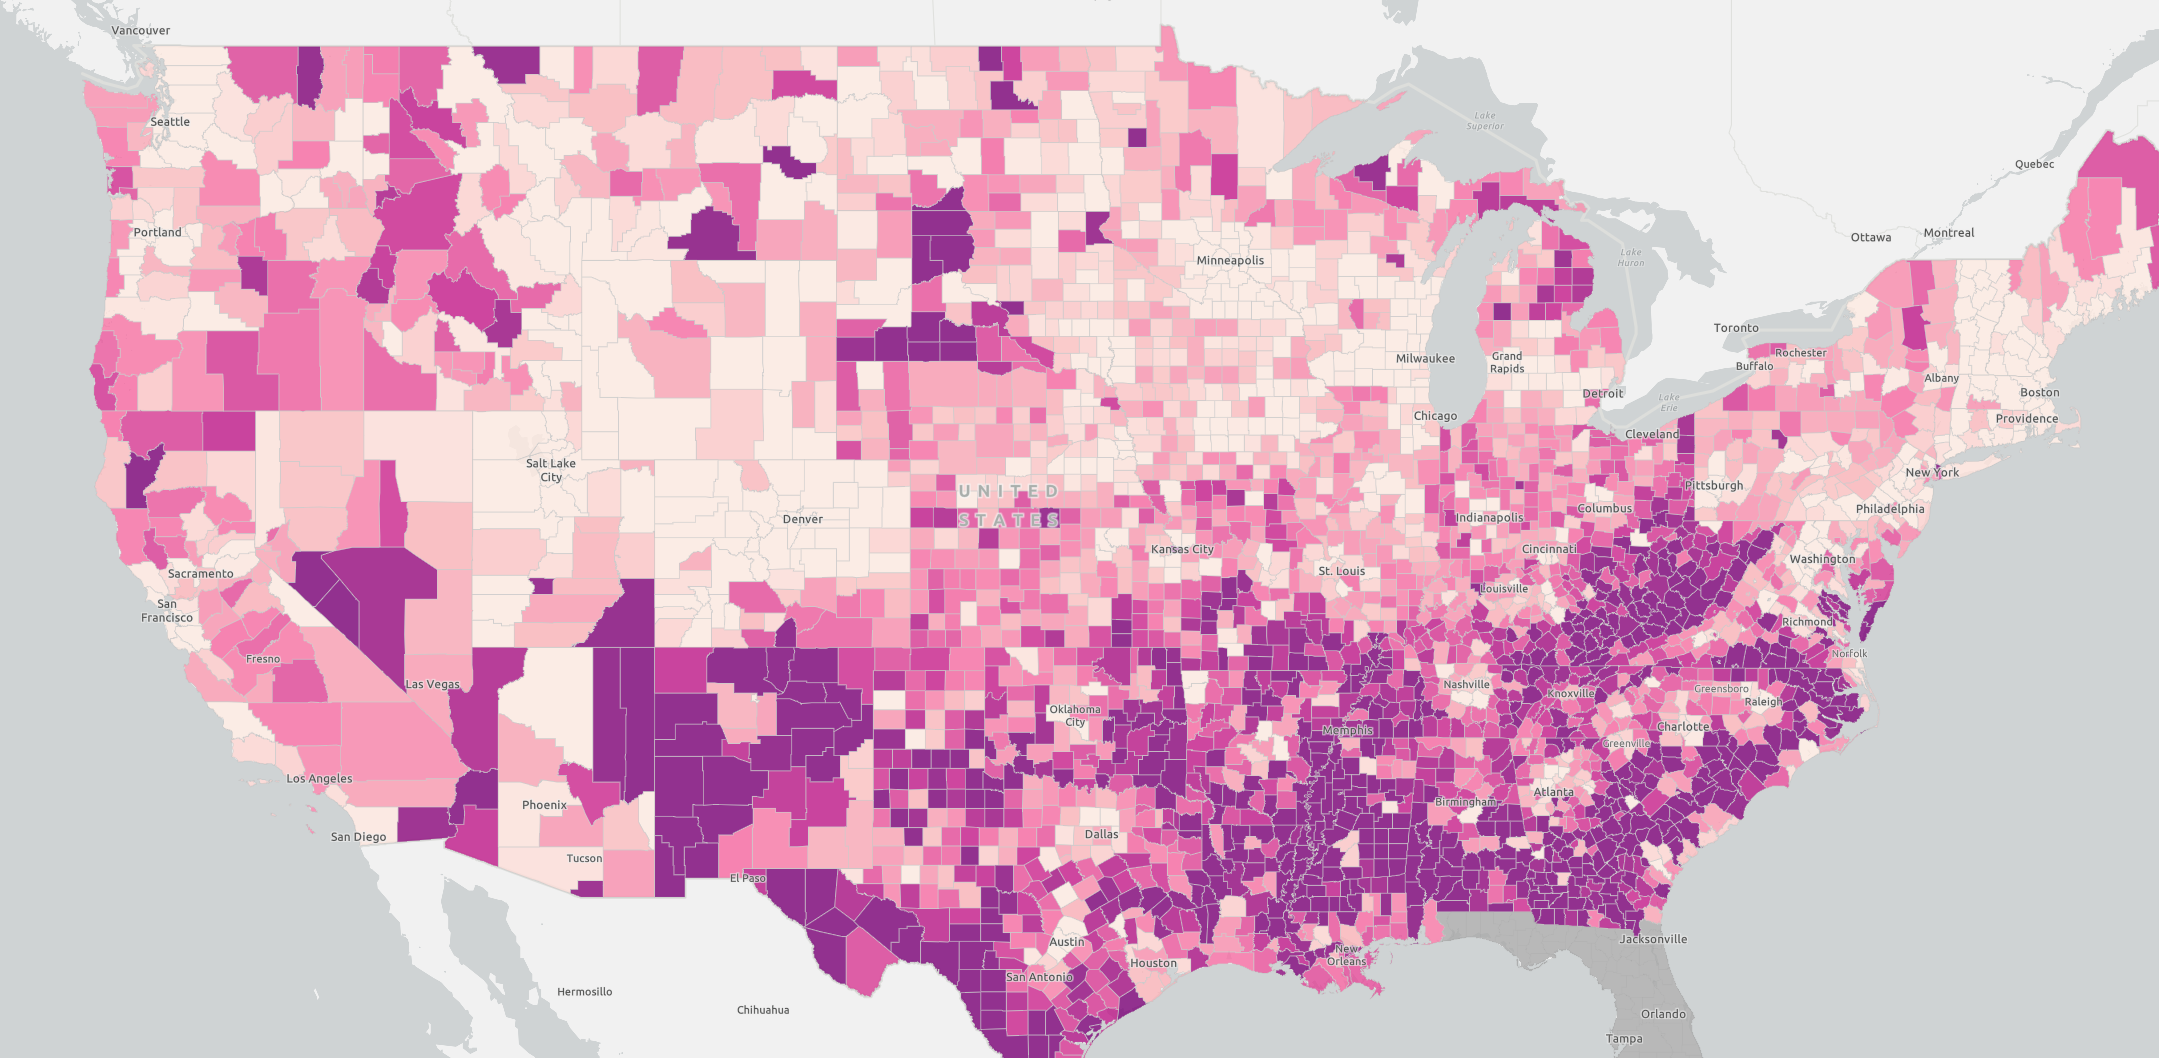
\includegraphics{places.png}

}

\caption{CDC Places Health Outcome Data: Diabetes Prevalence}

\end{figure}%
\end{frame}

\section{Case Studies}\label{case-studies}

\begin{frame}{Air Pollution Exposure Mapping}
\phantomsection\label{air-pollution-exposure-mapping}
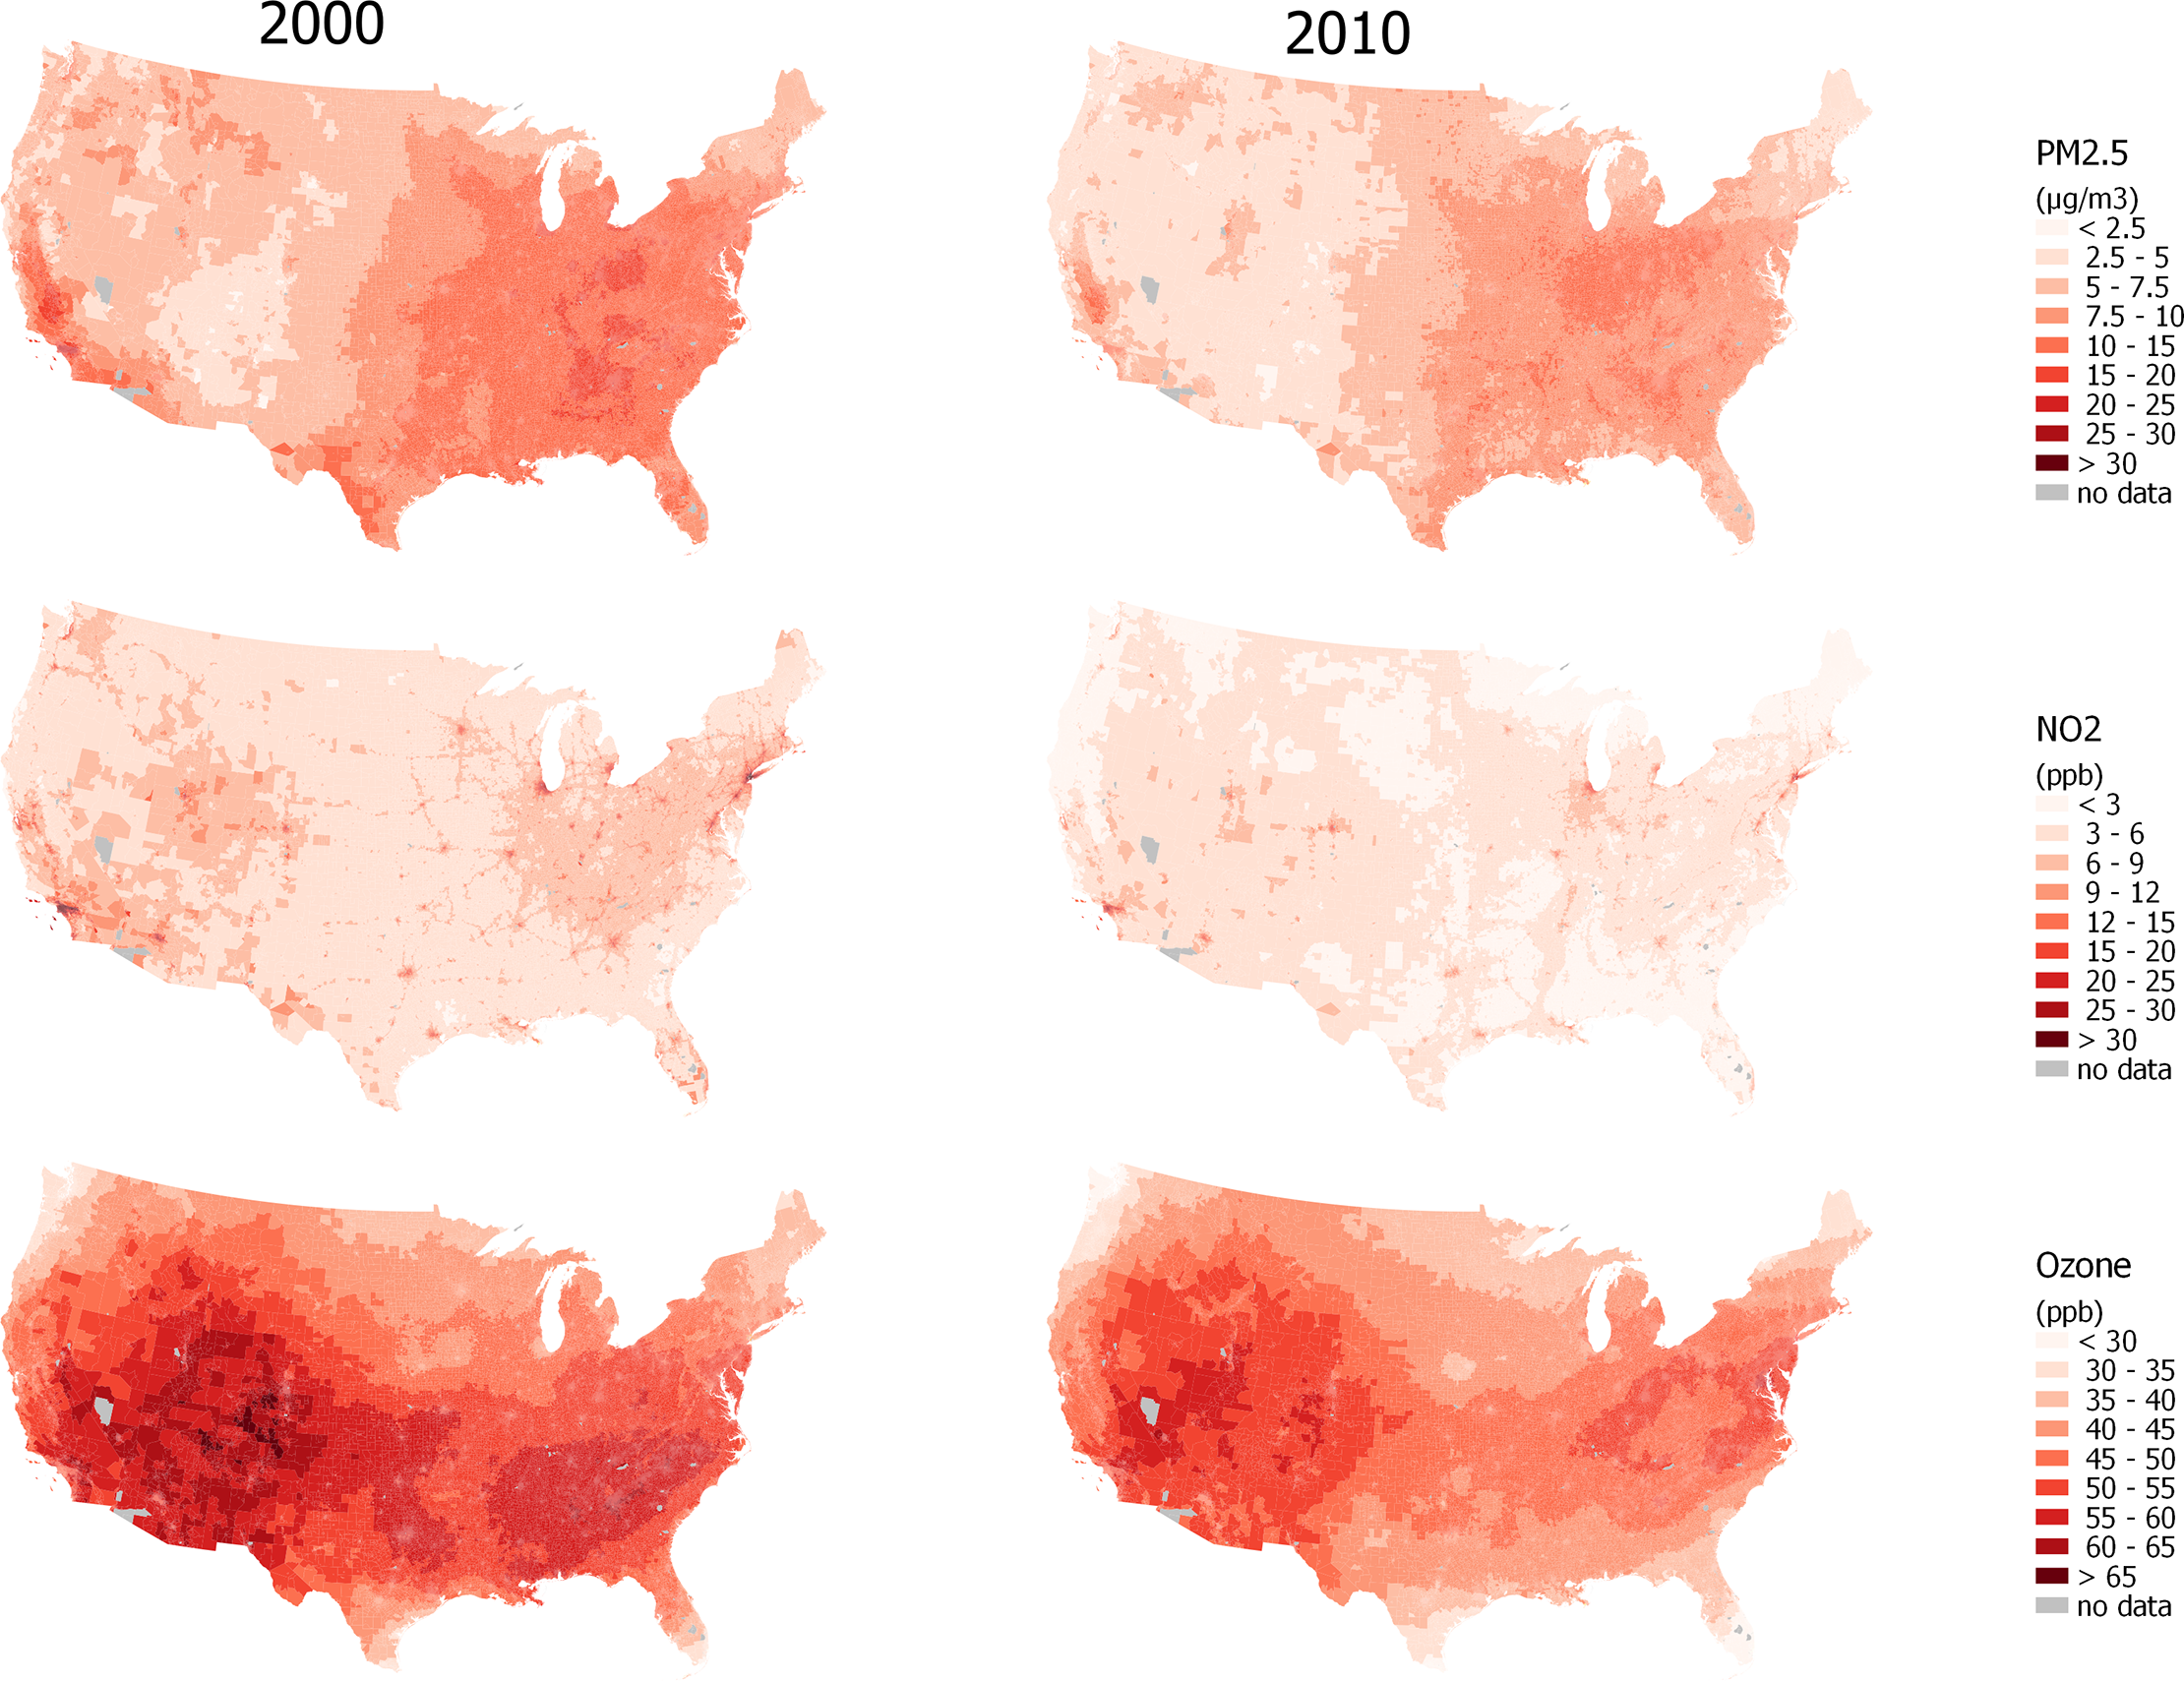
\includegraphics{spatial-PM25.png}
\end{frame}

\begin{frame}{Tale of Two Freeways}
\phantomsection\label{tale-of-two-freeways}
\begin{columns}[T]
\begin{column}{0.65\textwidth}
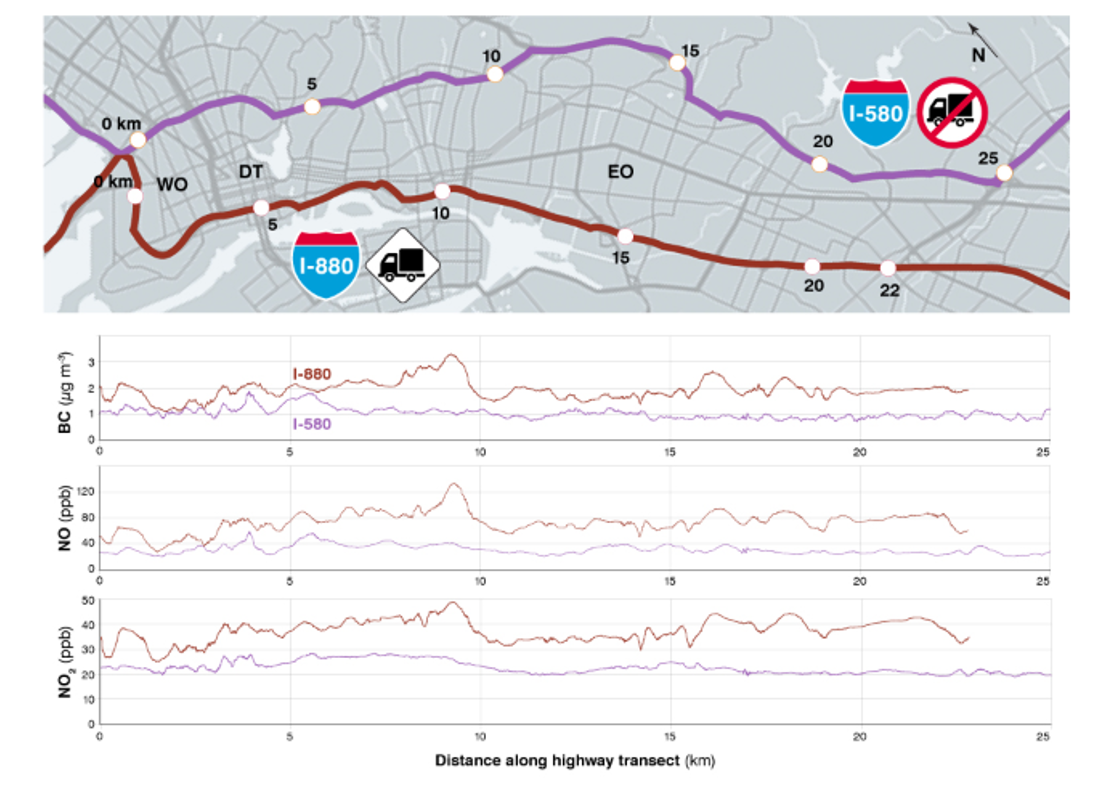
\includegraphics{two-freeways.png}
\end{column}

\begin{column}{0.35\textwidth}
\begin{itemize}
\item
  All measured pollutants were consistently higher on I-880 compared to
  I-580
\item
  I-580 has a heavy duty truck ban
\item
  Heavy duty trucks are forced onto I-880 to get to the Port of Oakland
\end{itemize}
\end{column}
\end{columns}
\end{frame}

\section{Source-to-Outcome}\label{source-to-outcome}

\begin{frame}{Source-to-Outcome Modeling}
\phantomsection\label{source-to-outcome-modeling}
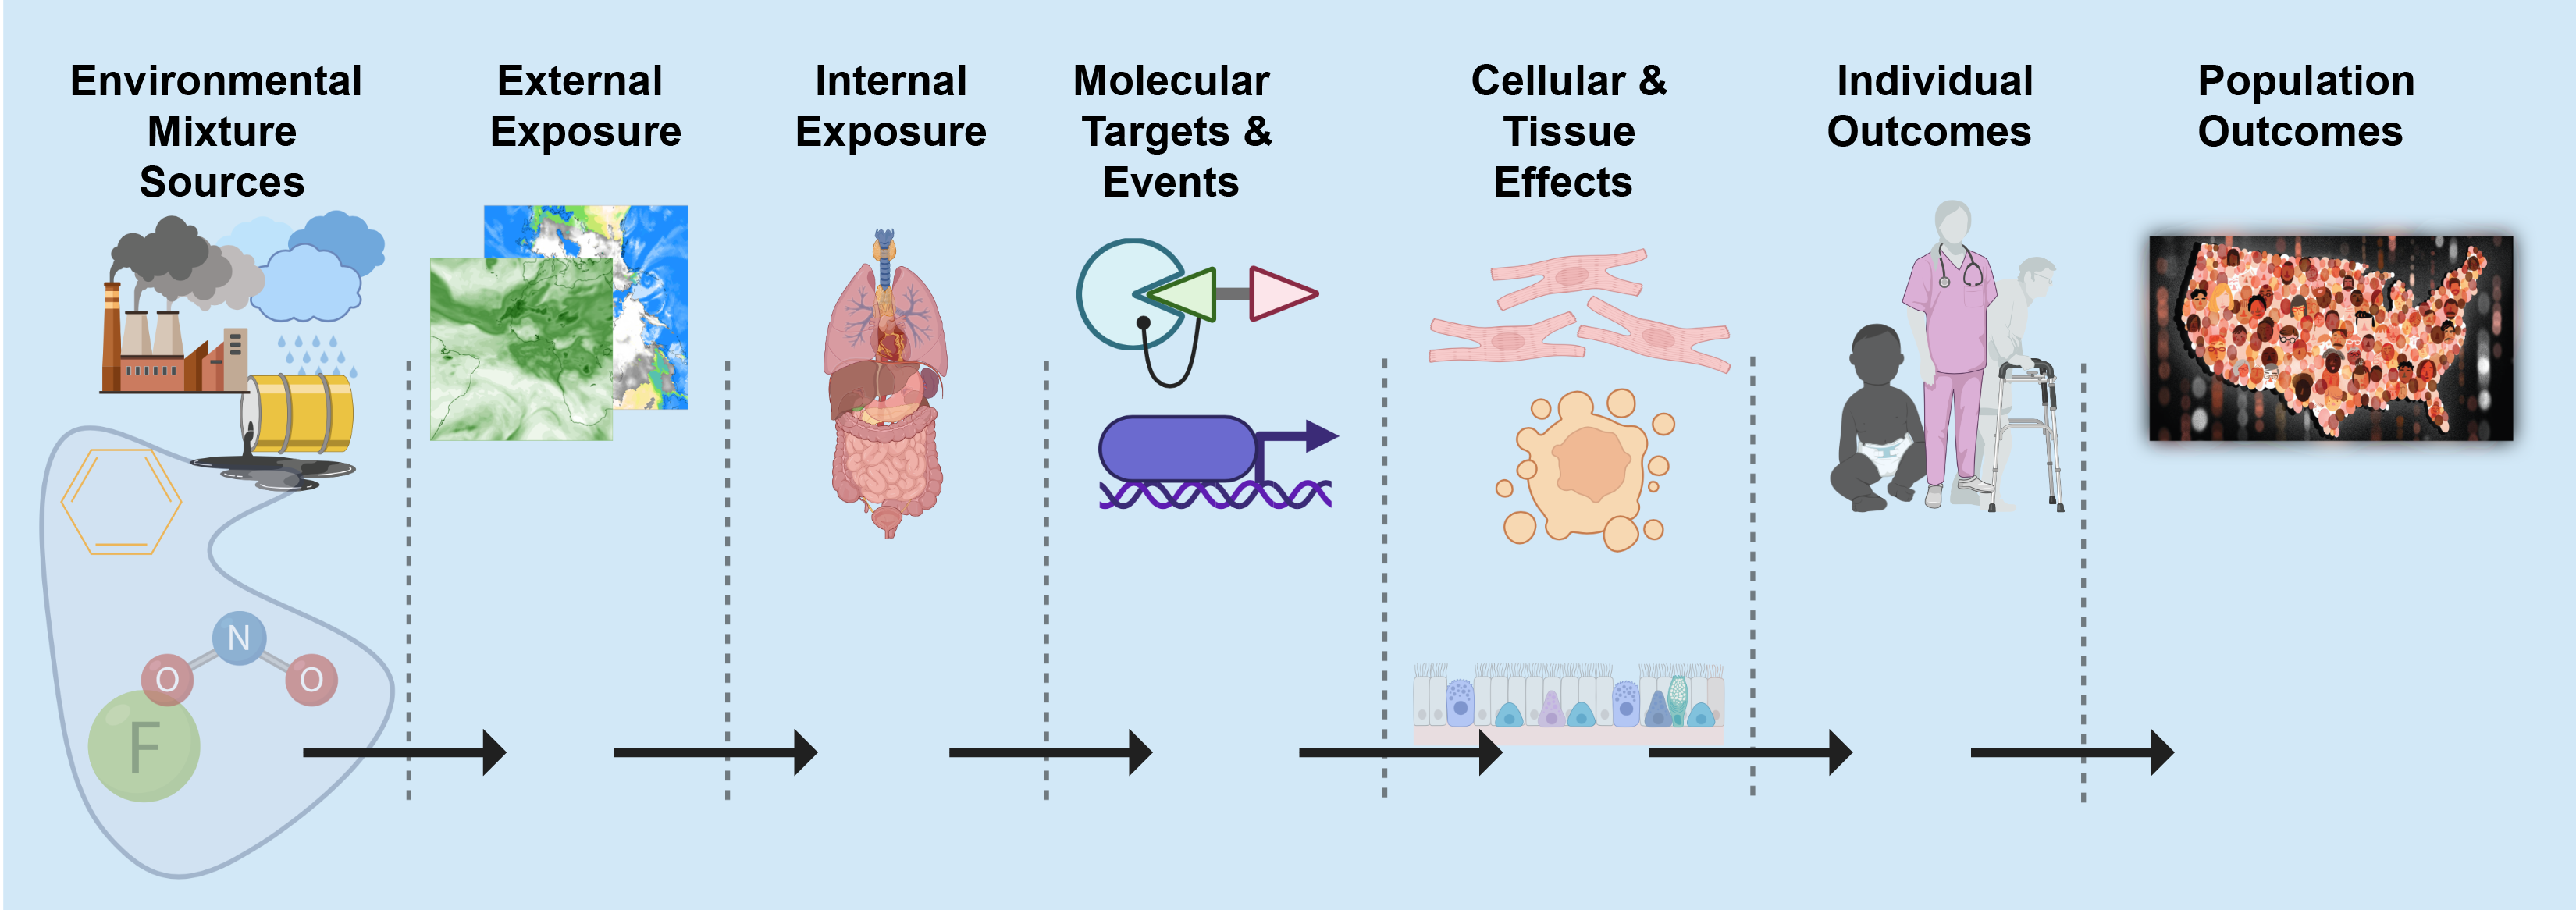
\includegraphics{../../presentations/20240214_SOT_ISES_Webinar/Exposome-Cascade.png}
\end{frame}

\begin{frame}{Source-to-Outcome Modeling}
\phantomsection\label{source-to-outcome-modeling-1}
\begin{itemize}
\item
  Source-to-Outcome is a framework for linking environmental sources to
  human health outcomes
\item
  The framework is based on the Aggregate Exposure Pathway (AEP) and
  Adverse Outcome Pathway (AOP) concepts
\end{itemize}
\end{frame}

\begin{frame}{Source-to-Outcome Modeling}
\phantomsection\label{source-to-outcome-modeling-2}
\begin{itemize}
\tightlist
\item
  Next generation risk of cumulative and total exposomic effects on
  human health
\item
  A balance between mechanistic and translational research
\item
  A framework for integrating multiple data sources and models
\item
  Incorporate biological and geospatial information on communities and
  individuals
\end{itemize}
\end{frame}

\begin{frame}{Getting Two Frameworks to Work Together}
\phantomsection\label{getting-two-frameworks-to-work-together}
\textbf{Aggregate Exposure Pathways}

\begin{itemize}
\tightlist
\item
  AEP is a comprehensive external analysis of source, media, and
  transformations
\end{itemize}

\textbf{Adverse Outcome Pathway}

\begin{itemize}
\tightlist
\item
  AOPs provide a linkage specific biological target, pathway or process
  by a stressor and an adverse outcome(s) considered relevant to risk
  assessment
\end{itemize}
\end{frame}

\begin{frame}{AEP-AOP}
\phantomsection\label{aep-aop}
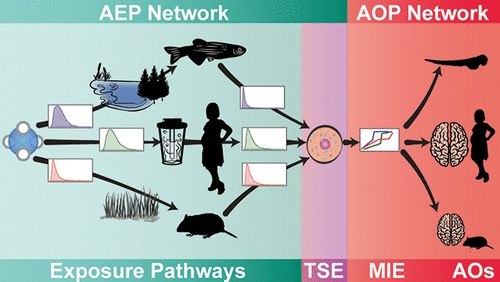
\includegraphics[width=0.8\textwidth,height=\textheight]{AEP-AOP-hines.jpeg}

Hines, D. E., Conolly, R. B., \& Jarabek, A. M. (2019)
\end{frame}

\begin{frame}[shrink]{GeoTox}
\phantomsection\label{geotox}
\begin{columns}[T]
\begin{column}{0.75\textwidth}
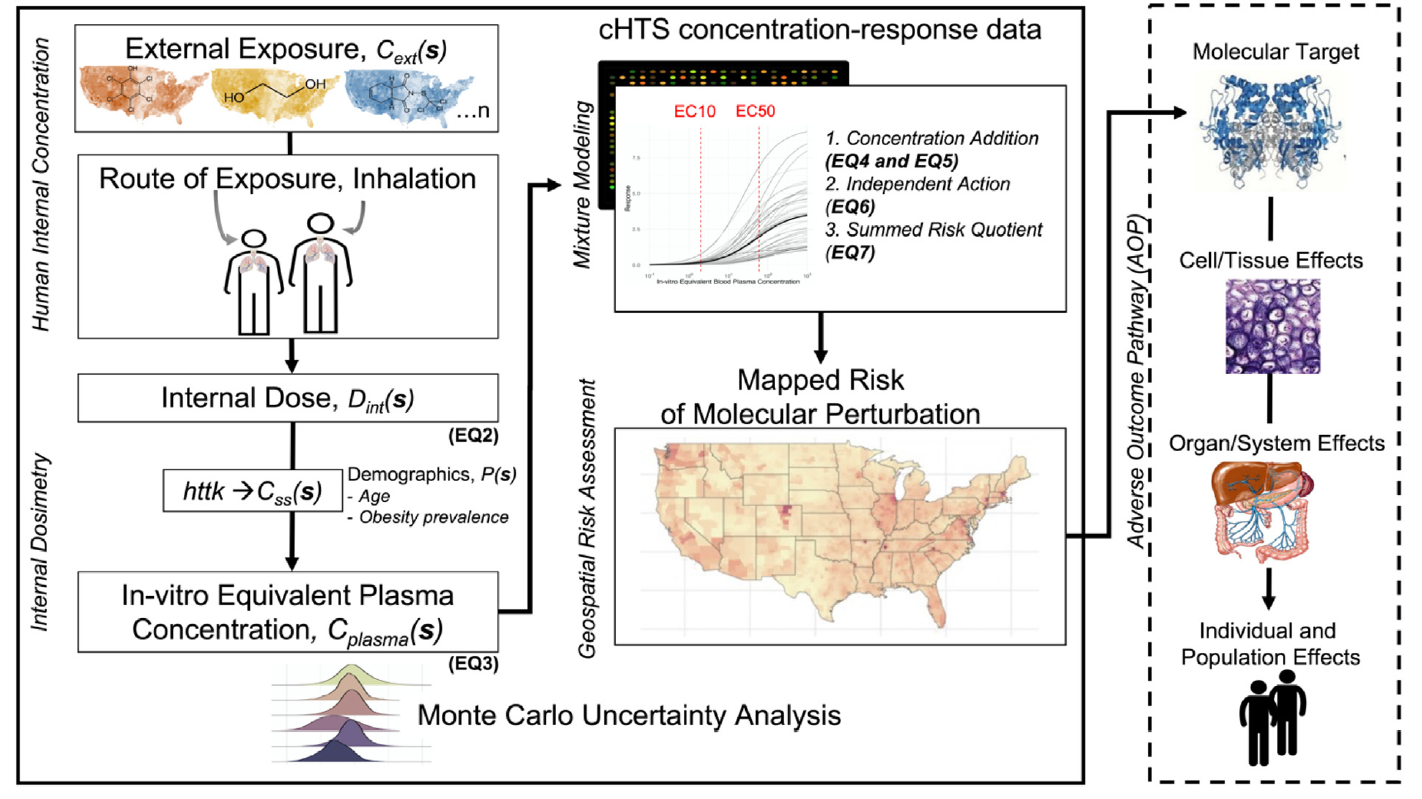
\includegraphics{GeoToxOutline.png}

Dr.~Kristin Eccles, Former Visiting Fellow in DTT and SET, Now at Health
Canada
\end{column}

\begin{column}{0.25\textwidth}
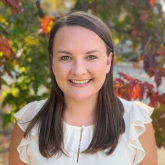
\includegraphics{../../presentations/20240214_SOT_ISES_Webinar/Eccles_headshot_resized.jpg}
\end{column}
\end{columns}
\end{frame}

\begin{frame}{GeoTox}
\phantomsection\label{geotox-1}
\begin{itemize}
\tightlist
\item
  Goal is to develop extensible, open-source software for facilitate
  source-to-outcome modeling (FAIR+)
\item
  Working with Drs. David Reif and Skylar Marvel (NIEHS/DTT)
\item
  Submitting to CRAN
\item
  Static website hosted via \{SET\}group website
\item
  Maintained, Documented, and Supported
\end{itemize}
\end{frame}

\begin{frame}[fragile,shrink]{GeoTox}
\phantomsection\label{geotox-2}
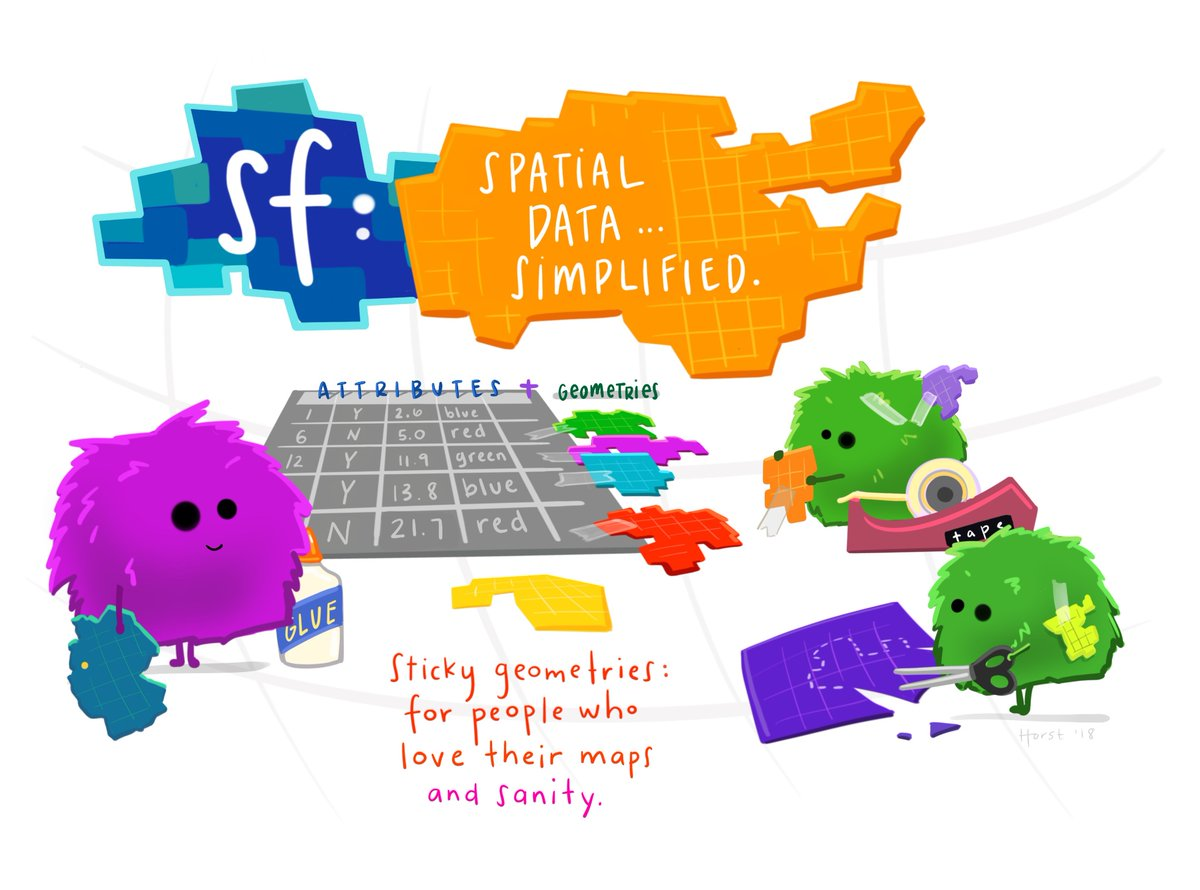
\includegraphics{sf-sticky.jpeg} \texttt{sf} package for spatial data in
R (Edzer Pebesma and others) (Illustration (c) 2018 by Allison Horst)
\end{frame}

\begin{frame}[shrink]{GeoTox}
\phantomsection\label{geotox-3}
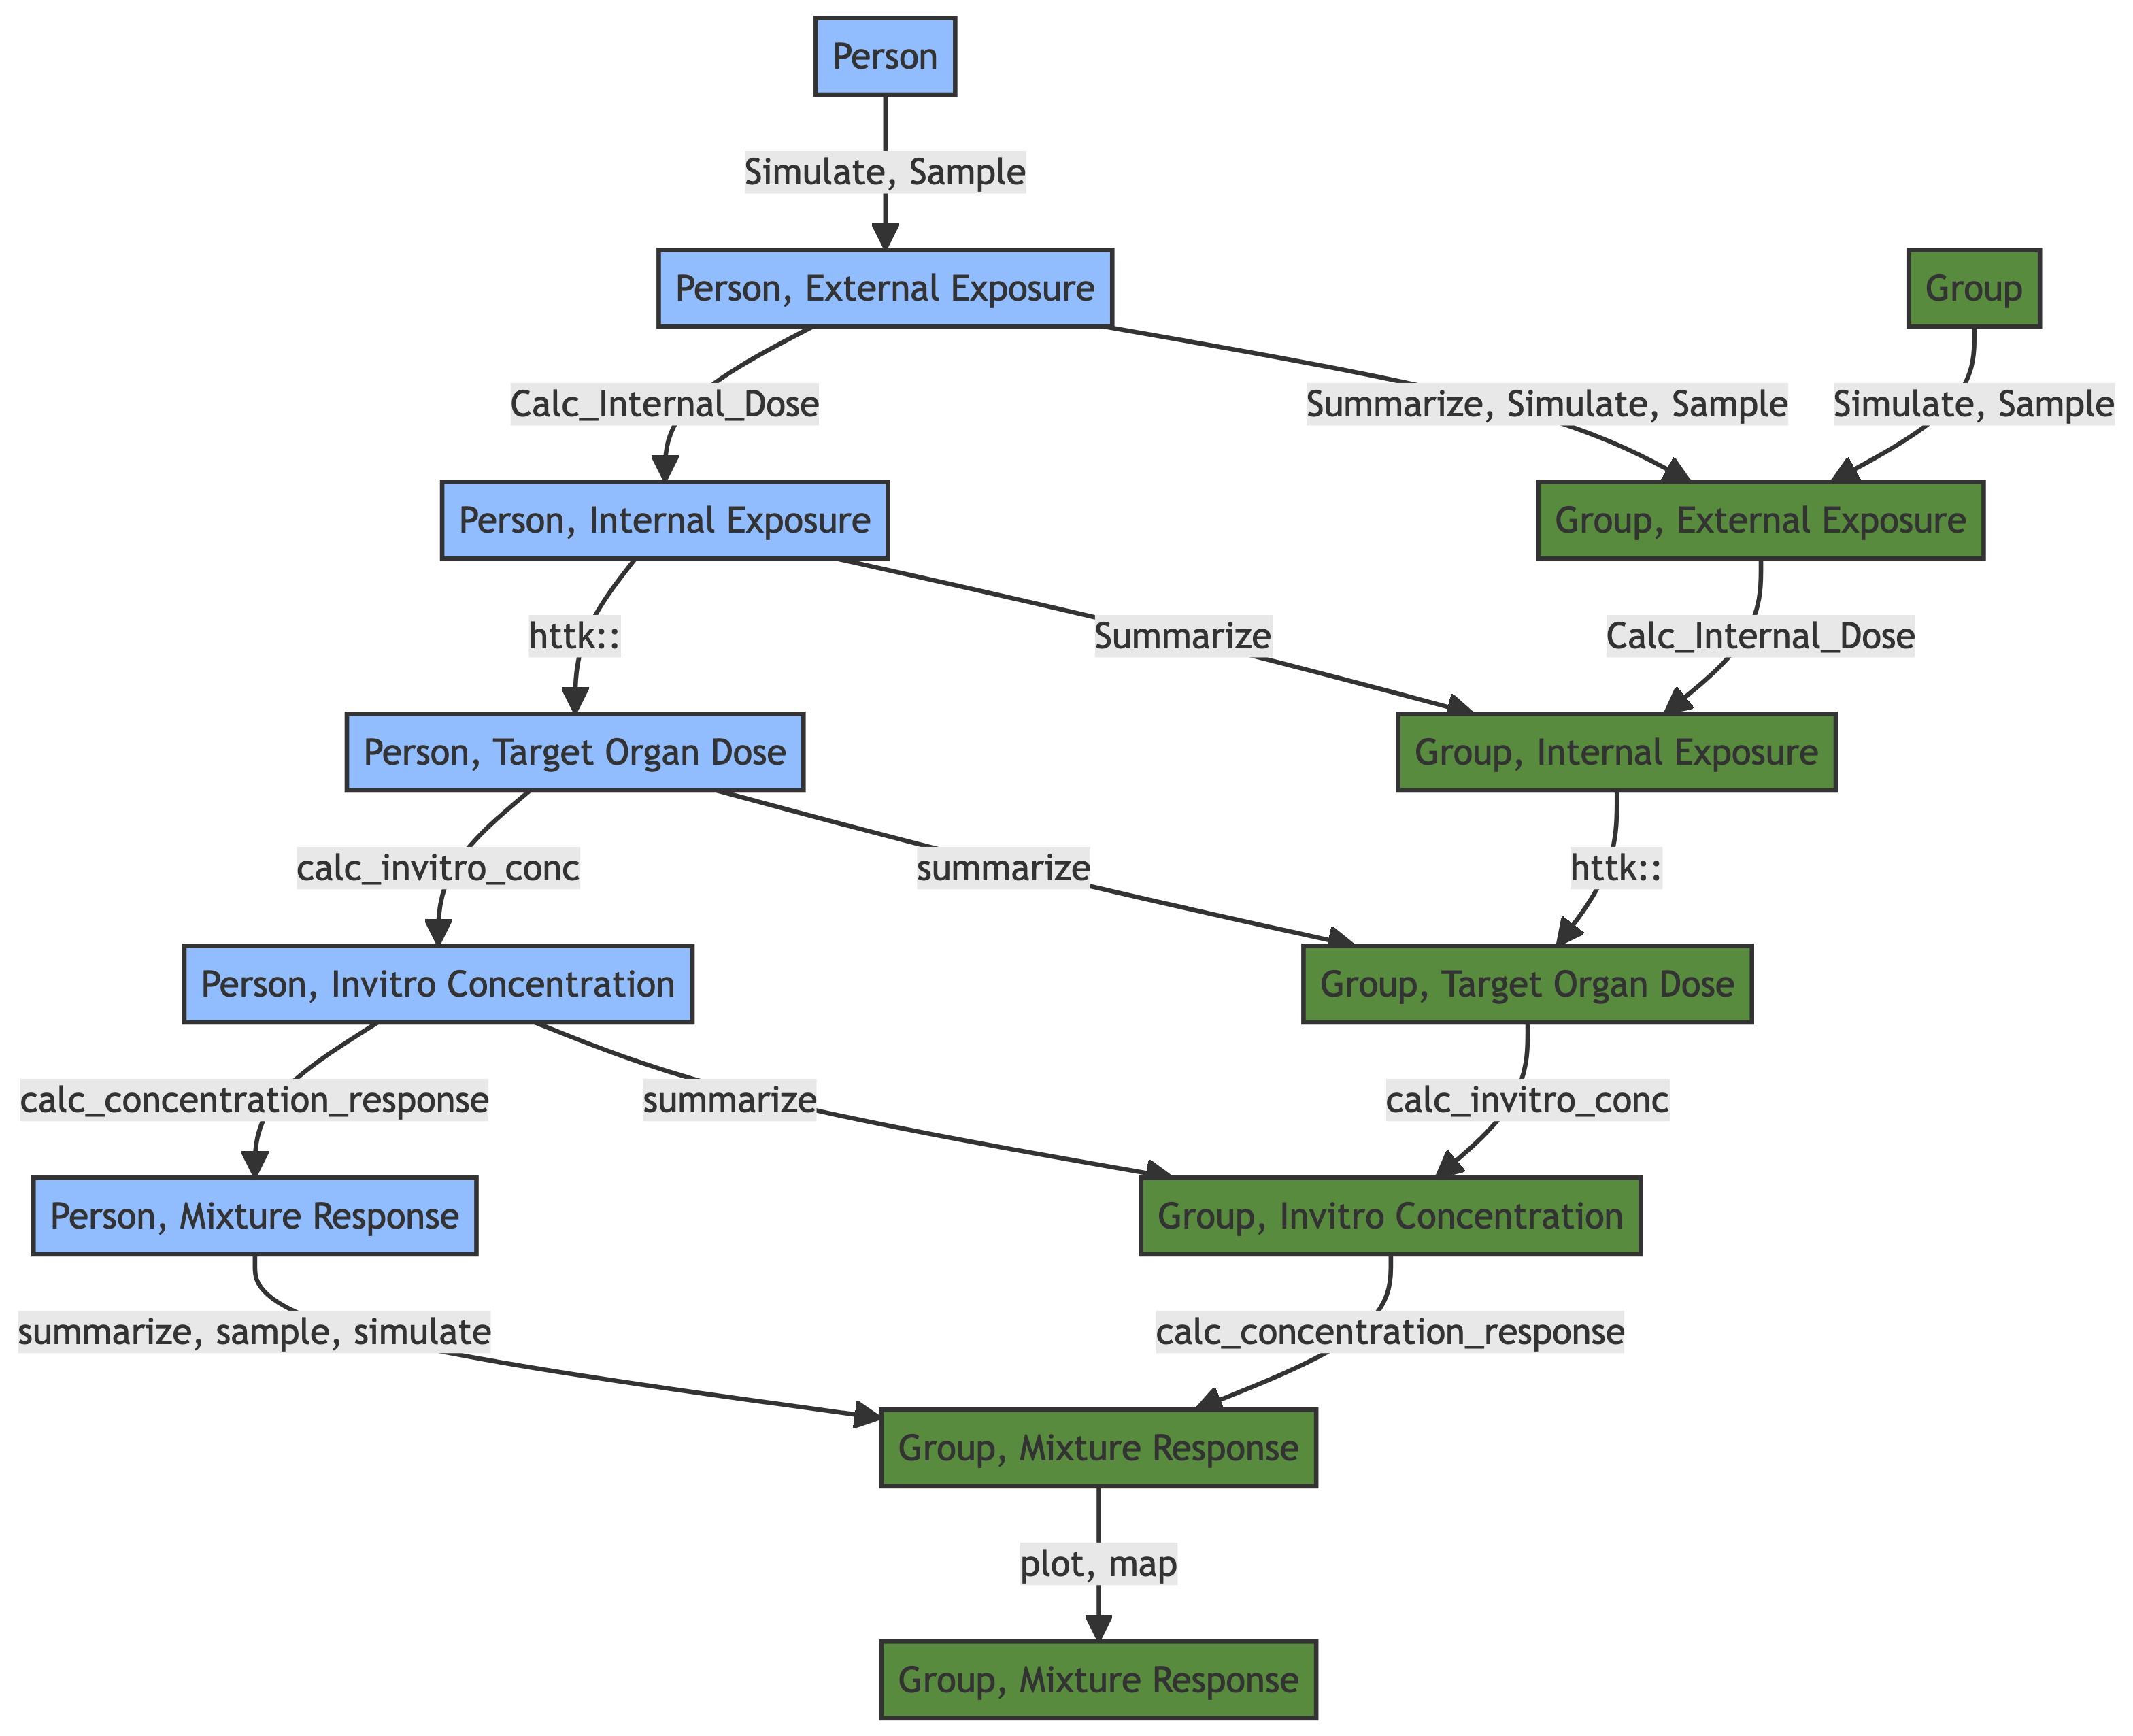
\includegraphics[width=9.87in,height=7.95in]{pegs_retreat_set_group_files/figure-beamer/mermaid-figure-1.png}
\end{frame}

\section{Conclusions}\label{conclusions}

\begin{frame}{Looking Forward}
\phantomsection\label{looking-forward}
\begin{itemize}
\item
  The tools for each step of the source-to-outcome modeling framework
  are available, but the integration is still a work in progress
\item
  The integration of these tools will allow for the development of a
  comprehensive source-to-outcome modeling framework that can be used to
  assess the risk of cumulative and total exposomic effects on human
  health
\end{itemize}
\end{frame}

\begin{frame}{Multiple Assays Informing an AOP}
\phantomsection\label{multiple-assays-informing-an-aop}
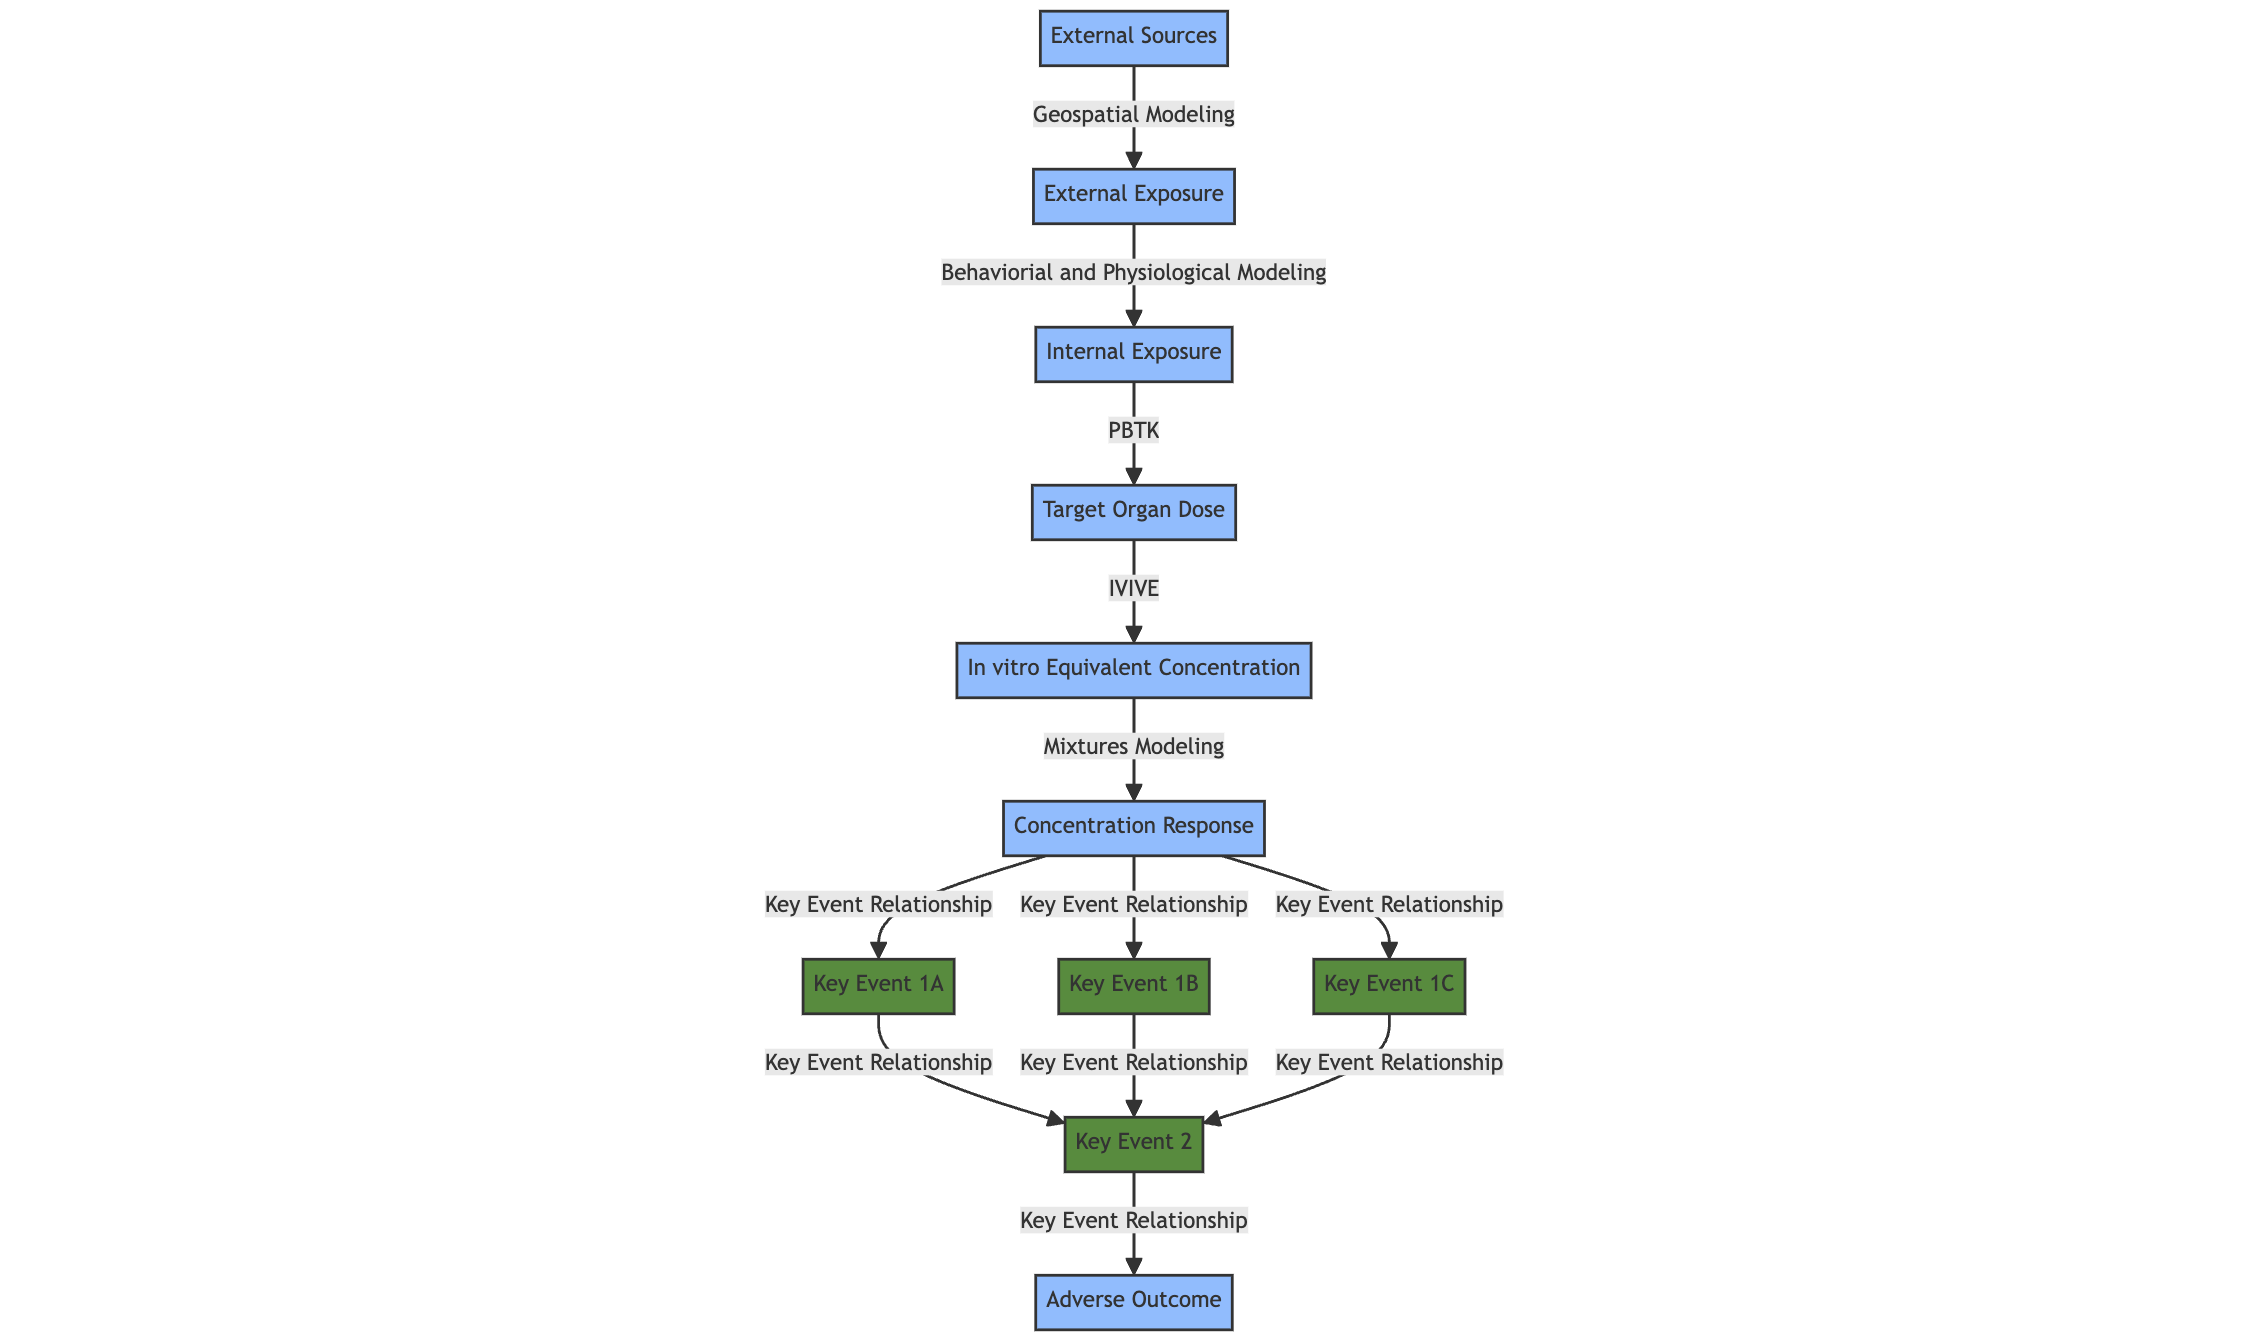
\includegraphics[width=1.15\textwidth,height=\textheight]{mermaid-diagram-2024-03-08-160259.png}
\end{frame}

\begin{frame}{Looking Forward}
\phantomsection\label{looking-forward-1}
\begin{itemize}
\item
  Incorporate more refined information on individual and
  population-level susceptibility to environmental exposures
\item
  It is going to be a massive code and software development challenge
\end{itemize}
\end{frame}

\begin{frame}{Looking Forward}
\phantomsection\label{looking-forward-2}
\begin{itemize}
\tightlist
\item
  Geospatial \textbf{exposures} are the foundation of a spatial, total
  exposome risk approach
\end{itemize}
\end{frame}

\begin{frame}{Acknowledgements}
\phantomsection\label{acknowledgements}
\begin{columns}[T]
\begin{column}{0.5\textwidth}
\begin{itemize}
\tightlist
\item
  Daniel Zilber
\item
  Mitchell Manware
\item
  Insang Song
\item
  Eva Marques
\item
  Ranadeep Daw
\item
  Mariana Alifa Kassien
\item
  Kristin Eccles
\item
  Melissa Lowe
\item
  Taylor Potter
\item
  Alvin Sheng
\end{itemize}
\end{column}

\begin{column}{0.5\textwidth}
\begin{itemize}
\tightlist
\item
  John Wambaugh
\item
  Alison Motsinger-Reif
\item
  David Reif
\item
  Skylar Marvel
\item
  Nicole Kleinstreuer
\item
  Julia Rager
\end{itemize}

\textbf{Funding:}

\begin{itemize}
\item
  NIEHS ZIA ES103368-02
\item
  Patient Centered Outcome Research Trust Fund (PCOR-TF)
\end{itemize}
\end{column}
\end{columns}
\end{frame}



\end{document}
